\documentclass[12pt,a4paper, pdftex]{elsarticle}
% artificial intelligence in medicine
\usepackage{amsmath}
\usepackage{amsfonts}
\usepackage{amssymb}
\usepackage{color}
\usepackage[utf8x]{inputenc}
\usepackage[T1]{fontenc}
%\usepackage{gentium}
\usepackage{mathptmx} % Use Times Font
\usepackage{natbib}
\usepackage[margin=0.8in]{geometry}
%\usepackage{graphics}
\usepackage[]{graphicx} % Required for including pictures
\usepackage[linkcolor=black,pdfborder={0 0 0}]{hyperref}
\hypersetup{colorlinks=true,urlcolor=blue,citecolor=blue, linkcolor=blue, breaklinks=true} % Format links for pdf
\usepackage{calc} % To reset the counter in the document after title pagehttps://www.overleaf.com/4569843284fwxryfmdhkyh
\usepackage{enumitem} % Includes lists
\usepackage{parskip}
\usepackage{url}
\frenchspacing % No double spacing between sentences
\linespread{1.2} % Set linespace

% Choose your own colour
\newcommand{\rmenote}[2][\textcolor{red}{\dagger}]{\textcolor{red}{$#1$}\marginpar{\color{red}\raggedright\tiny$#1$ #2}}
\newcommand{\rmeFIXME}[1]{\textcolor{red}{[\textbf{FIXME} \textsl{#1}]}}
\newcommand{\crjnote}[2][\textcolor{blue}{\dagger}]{\textcolor{blue}{$#1$}\marginpar{\color{blue}\raggedright\tiny$#1$ #2}}
\newcommand{\crjFIXME}[1]{\textcolor{blue}{[\textbf{FIXME} \textsl{#1}]}}
\newcommand{\manote}[2][\textcolor{magenta}{\dagger}]{\textcolor{magenta}{$#1$}\marginpar{\color{magenta}\raggedright\tiny$#1$ #2}}
\newcommand{\maFIXME}[1]{\textcolor{magenta}{[\textbf{FIXME} \textsl{#1}]}}

\usepackage{longtable}

%\PassOptionsToPackage{hyphens}{url}\usepackage{hyperref}
%\usepackage{xurl}
%\usepackage{soul}
\newcommand{\red}{\color{red}}

\newcommand{\beginsupplement}{%
        \setcounter{table}{0}
        \renewcommand{\thetable}{S\arabic{table}}%
        \setcounter{figure}{0}
        \renewcommand{\thefigure}{S\arabic{figure}}%
     }

\begin{document}

\begin{frontmatter}


\title{Using machine learning and clinical registry data to uncover variation in clinical decision making}

\author[inst1]{Charlotte James\corref{cor1}}

\author[inst1,inst2]{Michael Allen}

\author[inst1,inst3]{Martin James}

\author[inst4]{Richard Everson}

\affiliation[inst1]{organization={College of Medicine and Health},%Department and Organization
            addressline={University of Exeter}, 
            city={Exeter},
            country={UK}}

\affiliation[inst2]{organization={NIHR South West Peninsula Applied Research Collaboration (ARC)}}

\affiliation[inst3]{organization={Royal Devon and Exeter NHS Foundation Trust},%Department and Organization 
            city={Exeter},
            country={UK}}

\affiliation[inst4]{organization={Department of Computer Science},%Department and Organization
            addressline={University of Exeter}, 
            city={Exeter},
            country={UK}}
            
\cortext[cor1]{Corresponding author, charlotte.james@bristol.ac.uk}

\begin{abstract}
Clinical registry data contains a wealth of information on patients, clinical practice, outcomes and interventions. Machine learning algorithms are able to learn complex patterns from data. 
%
We present methods for using machine learning with clinical registry data to carry out retrospective audit of clinical practice. Using a registry of stroke patients, we demonstrate how machine learning can be used to: investigate whether patients would have been treated differently had they attended a different hospital; group hospitals according to clinical decision making practice; identify where there is variation in decision making between hospitals; characterise patients that hospitals find it hard to agree on how to treat.
%
Our methods should be applicable to any clinical registry and any machine learning algorithm to investigate the extent to which clinical practice is standardized and identify areas for improvement at a hospital level.


\end{abstract}



%%Research highlights
\begin{highlights}
\item We demonstrate how ML can be used for retrospective audit of clinical decision making.
\item When our methods are applied to a clinical registry of emergency stroke admissions we find significant variation in decision making.
\item Only 3\% of emergency stroke admissions who received thrombolysis would have received it at every hospital.
\item ML can be used to characterise typical patients where hospitals find it hard to agree on treatment.
\end{highlights}

\begin{keyword}

Clinical Registry \sep Machine Learning \sep Classification \sep Audit \sep Stroke

\end{keyword}

\end{frontmatter}



\section{Introduction}

Clinical registries are collections of information on people that have a specific disease, have experienced, or are at-risk of, an adverse health-related event or have been exposed to something that might have an adverse effect. They provide information on clinical practice, patient outcomes and the effect of interventions and are therefore useful for monitoring the course of disease, examining the effect of a treatment on patient outcome and measuring quality of care~\cite{gliklich2014registries}. 

In England the Healthcare Quality Improvement Partnership (HQIP), on behalf of the National Health Service (NHS), is responsible for over-seeing and commissioning more than 30 clinical audits (registries), which form the National Clinical Audit Programme. These collect and analyse registry data supplied by clinicians and are intended to be used for quality improvement by allowing the quality of care and services to be measured against agreed standards and for improvements to be made where necessary~\cite{burgess2011new}. The quantity and quality of data contained in these registries has the potential to provide insight into additional processes that can have an impact on patient outcome, such as clinical decision making. As decision making processes are complex and involve many interacting factors, standard statistical analyses are unlikely to capture this insight.  


 Machine learning algorithms are able to learn complex patterns from data. They have shown promise in many areas, including drug discovery~\cite{ekins2019exploiting}, precision medicine~\cite{cammarota2020gut}, medical diagnosis~\cite{olsen2020clinical, lee2020machine}, and clinical decision support~\cite{peiffer2020machine, buchlak2020machine} suggesting that, given the right data, ML algorithms can learn clinical decision making processes. As the data contained in clinical registries includes information on patients, clinical practice, treatment and outcomes, ML presents an opportunity to understand the decision making processes of clinicians, assess the extent to which these processes are standardized and, if not, uncover where decision making varies.

%

The national audit covering stroke is the Sentinel Stroke National Audit Programme (SSNAP)~\cite{party2015sentinel}. SSNAP collects longitudinal data on the processes and outcomes of stroke care up to 6 months post-stroke for more than 95\% of emergency stroke admissions to acute hospitals in England, Wales and Northern Ireland. Every year data from approximately 85,000 patients are collected. SSNAP publishes quarterly and yearly analysis of results on its website. Data from SSNAP has been previously used to investigate clinical decision making~\cite{parry2016care}, socioeconomic risk factors for stroke and their influence on care received and patient outcome~\cite{bray2018socioeconomic}, and temporal variation in stroke care~\cite{bray2016weekly}.

Stroke is a leading cause of death and disability worldwide which occurs when there is a blood clot or bleed in the brain preventing blood from reaching parts of the brain. Around 80-85\% of strokes are due to a blood clot (ischemic stroke). Thrombolysis is the only licensed drug treatment for acute ischemic stroke. It is critically time dependent: the longer the time window between stroke and administration, the less benefit to the patient. After 4.5 hours there is little or no benefit of thrombolysis~\cite{emberson2014effect}. In England, Wales and Northern Ireland, 11.1\% of patients with confirmed acute stroke receive thrombolysis, however there is considerable variation between hospitals, from 0\% to 24.5\%. Reasons for this variation are known to include slow uptake of the treatment and in-hospital delays to administration \cite{carter-jones_stroke_2011}; it is also possible that differences in clinical decision making play a part~\cite{de2018factors}.

To investigate whether variation in thrombolysis rates between hospitals is due, at least in part, to differences in clinical decision making we used a ML approach. Specifically, we trained ML algorithms to learn the decision making outcome in each hospital. The algorithms are trained using data that is available to the clinician and that the clinician would use to decide whether or not to administer thrombolysis to a patient. The algorithms predict the binary outcome, to thrombolyse (1) or not (0). By using ML to learn the decision making processes in a hospital, we are able to answer counterfactual, or `what if?', questions, such as `what if a patient had been admitted to a different hospital?'. This allows us to determine whether differences in clinical decision making contribute to the variation in thrombolysis rates observed between hospitals, and characterize patients that hospitals find it harder to agree how to treat.

While we focus on clinical decision making surrounding the use of thrombolysis for acute stroke, the methods we present should be applicable to any clinical registry data. These methods could be used with clinical registries to retrospectively assess variation in decision making between hospitals, group hospitals according to their decision making and characterise patients that clinicians find it difficult to agree how to treat. Uncovering differences in clinical practice using these methods may provide an opportunity to improve patient care by standardizing treatment across the board.

\section{Materials \& Methods}

\subsection{Data}

We used data from SSNAP collected over 3 years, from January 2016 to December 2018, corresponding to 246,676 emergency stroke admissions admitted to 180 acute care hospitals. We restricted our analysis to hospitals that admitted at least 100 patients during the 3 year time period and thrombolysed 10 or more. As thrombolysis is only considered to have a significant effect if given within 4.5 hours of stroke onset~\cite{emberson2014effect} and we are interested in emergency stroke admissions, only patients that had a stroke out of hospital and arrived in hospital within 4 hours of known stroke onset were included in the analysis. This resulted in 132 unique hospitals and 88,928 stroke patients, of which 26,257 (29.5\%) received thrombolysis. 

The data contained 47 features: admitting hospital (N=1), patient characteristics (N=5), pathway information (N=10), comorbidities (N=10), National Institutes of Health Stroke Scale (NIHSS) (N=16), other clinical information (N=4) and whether thrombolysis was given (N=1) (Table \ref{tab:S1}). 
The NIHSS is a 15 item neurological scale that is used by clinicians as a measure of stroke severity. It ranges from 0 to 42 and may be used to classify a stroke as mild (NIHSS 1-4), moderate (NIHSS 5-14), severe (NIHSS 15-24) or very severe (NIHSS > 25)~\cite{brott1989measurements}. Also present in the data is a patient's modified Rankin Scale (mRS) score before stroke, which is a measure of pre-stroke disability ranging from 0 to 5, with 0 corresponding to no prior disability and 5 meaning severely disabled.

Of the 47 features, 24 were missing for at least one patient (Table \ref{tab:S2}). If components of the NIHSS were missing they were replaced with 0 and if the time from arrival to brain scan ({\it Brain Imaging Time (minutes)}) was missing it was replaced with 9999, both of which force the probability of thrombolysis to be low. If a missing feature was binary it was coded as 'missing'. All binary and categorical variables were one-hot-encoded, with `missing' treated as a separate category. 


\subsection{Learning clinical decision making}

We used a ML approach to learn clinical decision making outcomes from the data. 

Specifically, we implemented a Random Forest (RF) which is an example of an ensemble learning algorithm composed of individual decision trees. We used RF as it is known to be robust and have a lower variance compared to a single decision tree. 
During training a RF will select a random sample of the training data with replacement and fit a decision tree to the sample. This process is repeated many times, the exact number being a parameter of the algorithm, to create an ensemble (or forest) of decision trees~\cite{breiman2001random}.

The RF is trained to perform a binary classification task: to decide whether a patient should be thrombolysed (class 1) or not (class 0). Each decision tree in the RF performs this classification task independently. A patient's final class is determined by averaging over the outcomes of all decision trees: if the average is less than the decision threshold, the patient is assigned class 0 (not thrombolysed) else the patient is assigned class 1 (thrombolysed).

To implement the RF, we used Python's sci-kit learn library~\cite{pedregosa2011scikit} incorporating stratified 10-fold cross-validation: the data was split into a training set (90\%) and validation set (10\%) ten times, such that each patient is in the validation set exactly once. The RF was fit to the training set at each fold and the validation set was used to assess performance. Final performance measures were determined by averaging over those for each fold.

\subsection{Hospital models}

We divided our data into separate hospitals and trained an RF on patients from each hospital. Each of these RFs learn the decision making within a single hospital during training. We again used stratified 10-fold cross-validation and assessed how well each model was able to learn the decision making at each hospital. The decision threshold of each model was calibrated such that the predicted positive rate (i.e. fraction of patients predicted to be given thrombolysis) was equal to the true positive rate.


\subsection{Assessing variation in decision making}

To investigate how decision making varies between hospitals, we again trained RFs on patients from each hospital, using all patients from that hospital for training, as opposed to 10-fold cross validation. We subsequently took all other patients in our data set and applied each hospital's RF to every patient: the classification given by each RF represents what would have happened if a patient had been treated at that hospital.

\subsection{Grouping hospitals by decision making}

To find hospitals with similar decision making processes, we set aside a representative cohort of 10,000 patients. We trained an RF on patients from each hospital selected from the remaining 78,928 patients. Each RF was applied to the cohort of patients to determine whether or not each patient would have been thromoblysed had they attended each hospital. We computed the pairwise Hamming distance, $D_H$, between the predicted outcomes for every pair of hospitals.  The Hamming distance is the proportion of patients on which the two hospital models disagree on the outcome: if $D_H$ is close to $0$ the hospitals would make similar decisions, whereas if it is close to $1$ their modelled decision making processes are different.

\section{Results}

%------------------------ TABLE 1 ------------------------------
\subsection{Population characteristics} 
    \begin{table}[h!]
        \centering
        \begin{tabular}{|l|c|c|}
        \hline
        {\bf Measure$^1$} & {\bf Thrombolysed N = 26257} & {\bf Not Thrombolysed N = 62671}  \\
        \hline
        Age (years) & 73 (14) & 76 (14)\\
        Female (N, \%) & 12084 (46) & 30796 (49)\\
        White (N, \%) & 22861 (87) & 55660 (89)\\
        Onset to Arrival (minutes) & 97 (46) & 117 (54) \\
        Arrival to Imaging (minutes) & 23 (20)  & 157 (1095)$^2$\\
        NIHSS & 11.6 (7.0) & 8.4 (8.4)\\
        Facial Palsy & 1.2 (0.9) & 0.8 (0.8)\\
        Dysarthria & 1.0 (0.8) & 0.7 (0.8)\\
        Best Language & 1.1 (1.1) & 0.7 (1.1) \\
        Rankin before Stroke & 0.7 (1.2) & 1.2 (1.5) \\
        \hline
        \end{tabular}
        \caption{Population characteristics stratified by outcome for patients in the treatment pathway. $^1$Values correspond to mean (std) unless otherwise stated. $^2$Standard deviation affected by imputation method}.
        \label{tab:1}
    \end{table}

%------------------------ TABLE 1 ------------------------------
Population characteristics are displayed in Table \ref{tab:1}. Patients that were thrombolysed were, on average, younger (mean 73 years), arrived at the hospital in less time (mean 97 mins), had brain imaging scans faster (mean 23 mins), had more severe stroke (mean NIHSS 11.6) and lower levels of disability (mean rankin 0.7) compared to those that were not thrombolysed. 


\subsection{Learning clinical decision making}



%------------------------ TABLE 2 ------------------------------
    \begin{table}[h!]
        \centering
        \begin{tabular}{|l|c|c|}
        \hline
        {\bf Performance Measure} & {\bf Combined Model$^{1,2}$}  & {\bf Hospital Models$^3$} \\
        \hline
        Accuracy & 84.3 (83.6 - 84.7) & 84.5 (76.1 - 95.2)\\
        Sensitivity & 0.69 (0.67 - 0.70) & 0.72 (0.43 - 0.86)\\
        Specificity & 0.91 (0.90 - 0.91) & 0.86 (0.76 - 0.97)\\
        False positive rate & 0.09 (0.09 - 0.10) & 0.11 (0.03 - 0.24)\\
        False negative rate & 0.31 (0.30 - 0.33) & 0.28 (0.14 - 0.56)\\
        Positive predictive value & 0.69 (0.67 - 0.70) & 0.72 (0.43 - 0.86)\\
        Negative predictive value & 0.91 (0.90 - 0.91) & 0.89 (0.76 - 0.97)\\
        Positive rate & 0.27 (0.26 - 0.27) & 0.29 (0.06 - 0.50)\\
        AUC$^4$ & 0.91 (0.91 - 0.92) & 0.90 (0.80 - 0.97)\\
        \hline
        \end{tabular}
        \caption{Performance measures of Random Forest algorithm trained on data from all hospitals together with one-hot encoding of hospital ID (Combined Model) and each hospital separately (Hospital Models) $^1$For a decision threshold of 0.5. $^2$Values correspond to mean (range) of 10 folds $^3$Values correspond to mean (range) of all 132 hospital models. $^4$ AUC independent of decision threshold}
        \label{tab:2}
    \end{table}
%------------------------ TABLE 2 ------------------------------
%\crjFIXME{CJ to add AUC to table 2 and text}

Model performance is described in Table \ref{tab:2}: the RF trained on all patients performed well with a mean accuracy of 84.3\% (range 83.6 - 84.7) and AUC of 0.91 (range 0.91 - 0.92). An accuracy of 85\% means that 15\% of patients were misclassified (Combined Model, Table \ref{tab:2}). If clinical decision making was consistent both within and between hospitals we would expect misclassified patients to lie close to the decision boundary: these patients represent borderline decisions. To verify this, we looked at the probability distribution for misclassified patients, where the probability is the average outcome over all trees in the RF. From Figure \ref{fig:hist} it is clear that while the distribution is approximately centred on the decision threshold there is a significant proportion of patients who were confidently misclassified: the probability of receiving thrombolysis is close to 0 or 1. This shows that not all misclassified patients represent borderline decisions and therefore supports our hypothesis that there is variation in clinical decision making: a confident misclassification means that there was a similar patient in the training data who was treated differently. % \manote{Not sure this latter point is true?}
%{\bf add rate of confident misclassification?} 

\begin{figure}[h!!!]
\centering
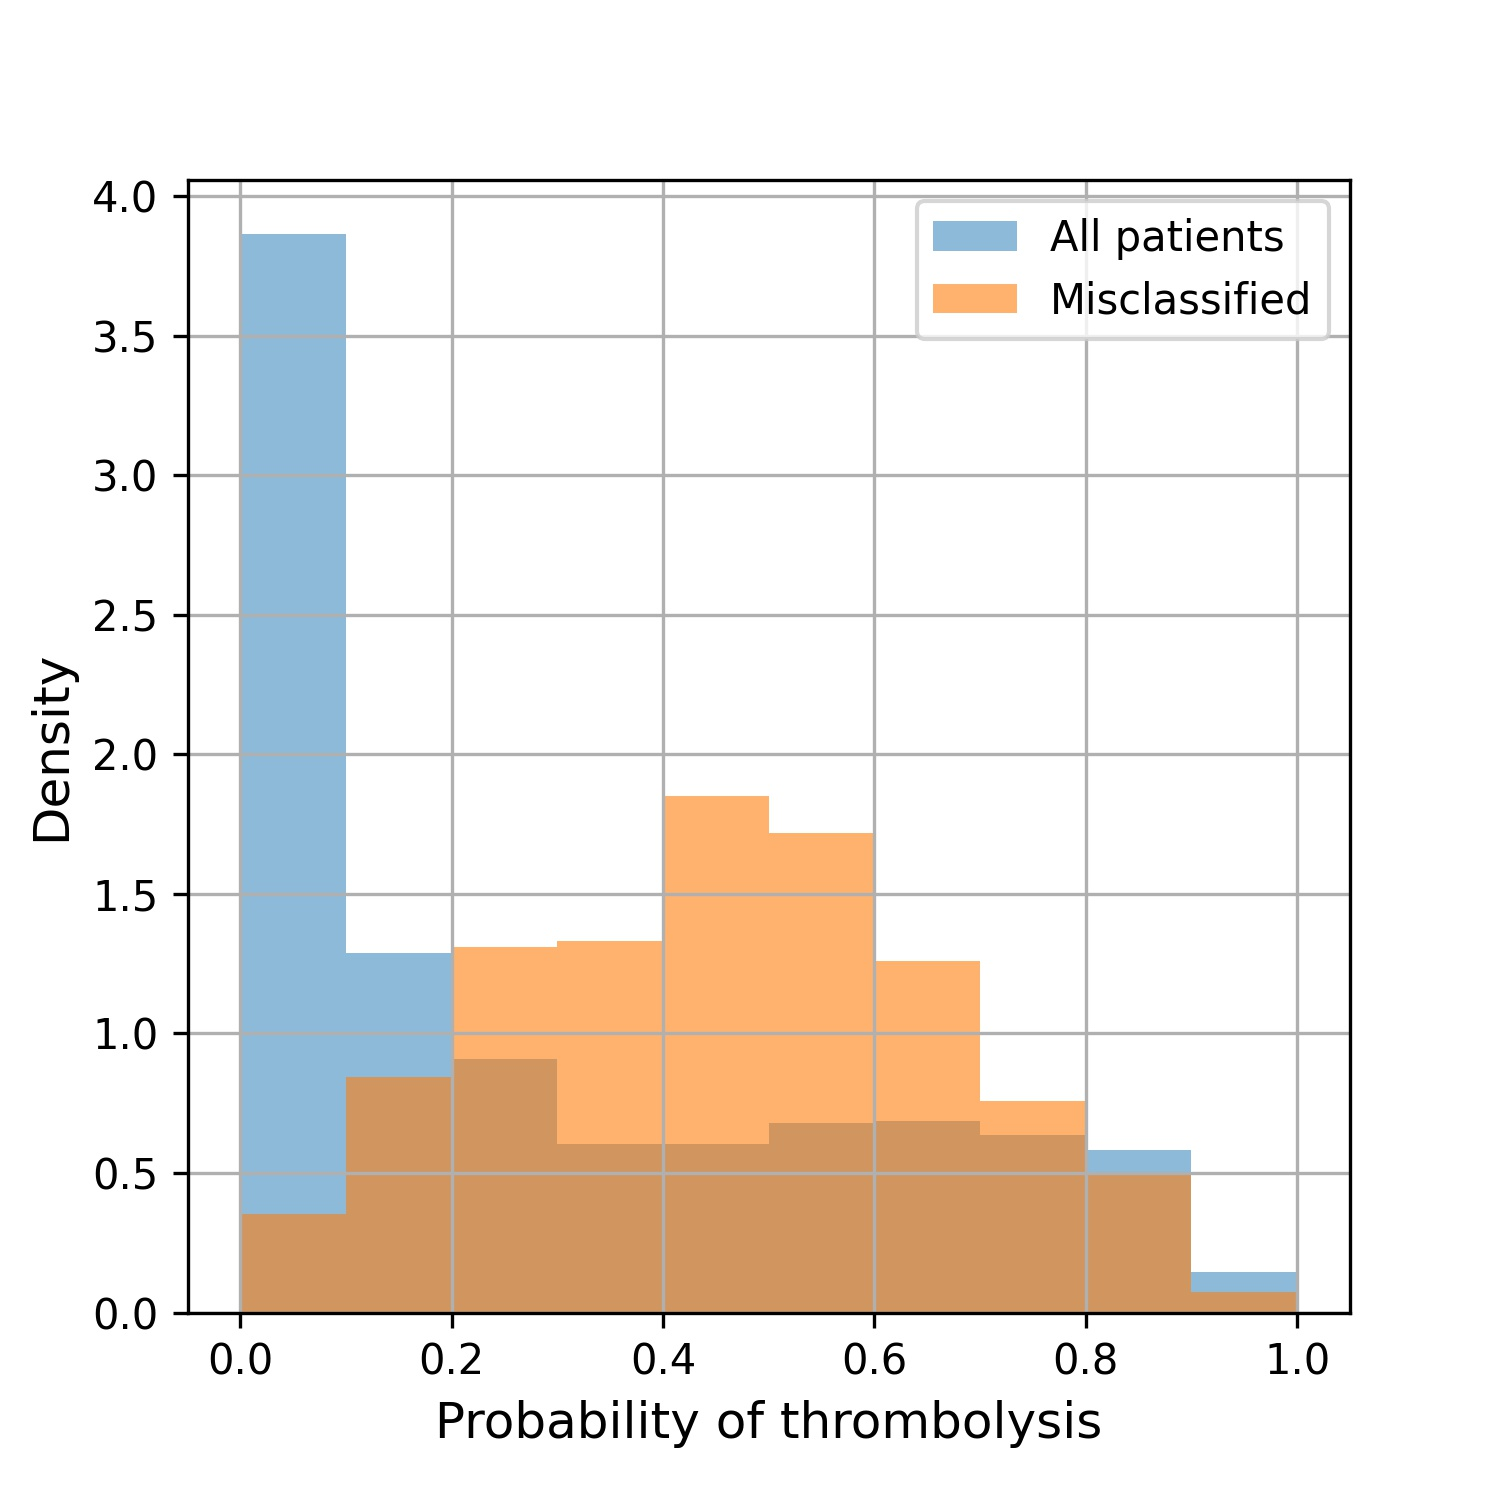
\includegraphics[width=10cm]{figures/probability_histogram.jpg}
\caption{Probability distribution for patients misclassified by a Random Forest algorithm trained on data from all hospitals together.}
\label{fig:hist}
\end{figure}


\subsection{Hospital models}

In order to understand sources of variation in decision making between hospitals, we trained separate RFs on the patients from each of the 132 hospitals. On average, individual hospital models perform similarly to the combined model (Table \ref{tab:2}). However, for each measure there is a range of values: the lowest performing hospital model has an accuracy of 76.1\% and AUC of 0.80, which is significantly lower than the accuracy and AUC of the combined model (84.3\% and 0.91). The range of values of the performance measures may be explained by variation in hospital size and thrombolysis rates. The performance of each hospital model will be affected by both the amount of data (hospital size) and class balance (thrombolysis rate): hospitals with a smaller number of patients and lower thrombolysis rate are less likely to have well calibrated models.

We assessed how well hospital models were calibrated by plotting a calibration curve for each model (Figure \ref{fig:calibration}a). If a model is perfectly calibrated, the proportion of a set of patients that are assigned an equal probability of receiving thrombolysis by the model, that go on to receive thrombolysis, should be equal to the probability: i.e. out of all patients the model assigns a 60\% chance of receiving thrombolysis to, 60\% of the patients should receive it. 


From Figure \ref{fig:calibration}a, most hospital models are well calibrated, however some do not output probabilities over the whole range, or are not well calibrated at higher probabilities (Figure \ref{fig:calibration}b). In order to improve model calibration we applied Platt Scaling~\cite{platt1999probabilistic}, fitting a logistic regression to the probabilities output by each hospital model. After applying Platt Scaling, the model calibration curves are closer to that of the perfectly calibrated model (black dashed line, Figure \ref{fig:calibration}c). Figure \ref{fig:uncalibrated} shows how hospitals with models that were not well calibrated compare to other hospitals in terms of number of patients and thrombolysis rate. From this it is clear that hospitals that have both fewer patients and lower thrombolysis rates are less likely to be well calibrated. This may be attributed to the training data for these hospital models being both smaller in size and more imbalanced.

As with the combined model, hospital models also confidently misclassify patients (Figure \ref{fig:missed}). In this case, confident misclassifications represent cases were a patient was treated differently to what would be expected in that hospital: for a confident misclassification to occur, a similar patient that was treated differently must be present in the training data. However, the reason that these patients were treated differently to the norm for the hospital they attended is likely not captured in the data and will not be explored further.

\subsection{Assessing variation in decision making}

Using hospital models, each trained on all patients from a single hospital, we determined how each patient in the dataset would have been treated had they attended a different hospital. We found that it is much easier for hospitals to agree who not to thrombolyse than who to give thromobolysis to (Figure \ref{fig:aggree}). Specifically 80\% of hospitals agree not to thrombolyse 85\% of patients that did not receive thrombolysis, whereas only 60\% of patients who did receive thrombolysis would have received it at 80\% of hospitals. Only 3\% of patients that were given thrombolysis would have received it at every hospital.

\begin{figure}[ht!]
\centering
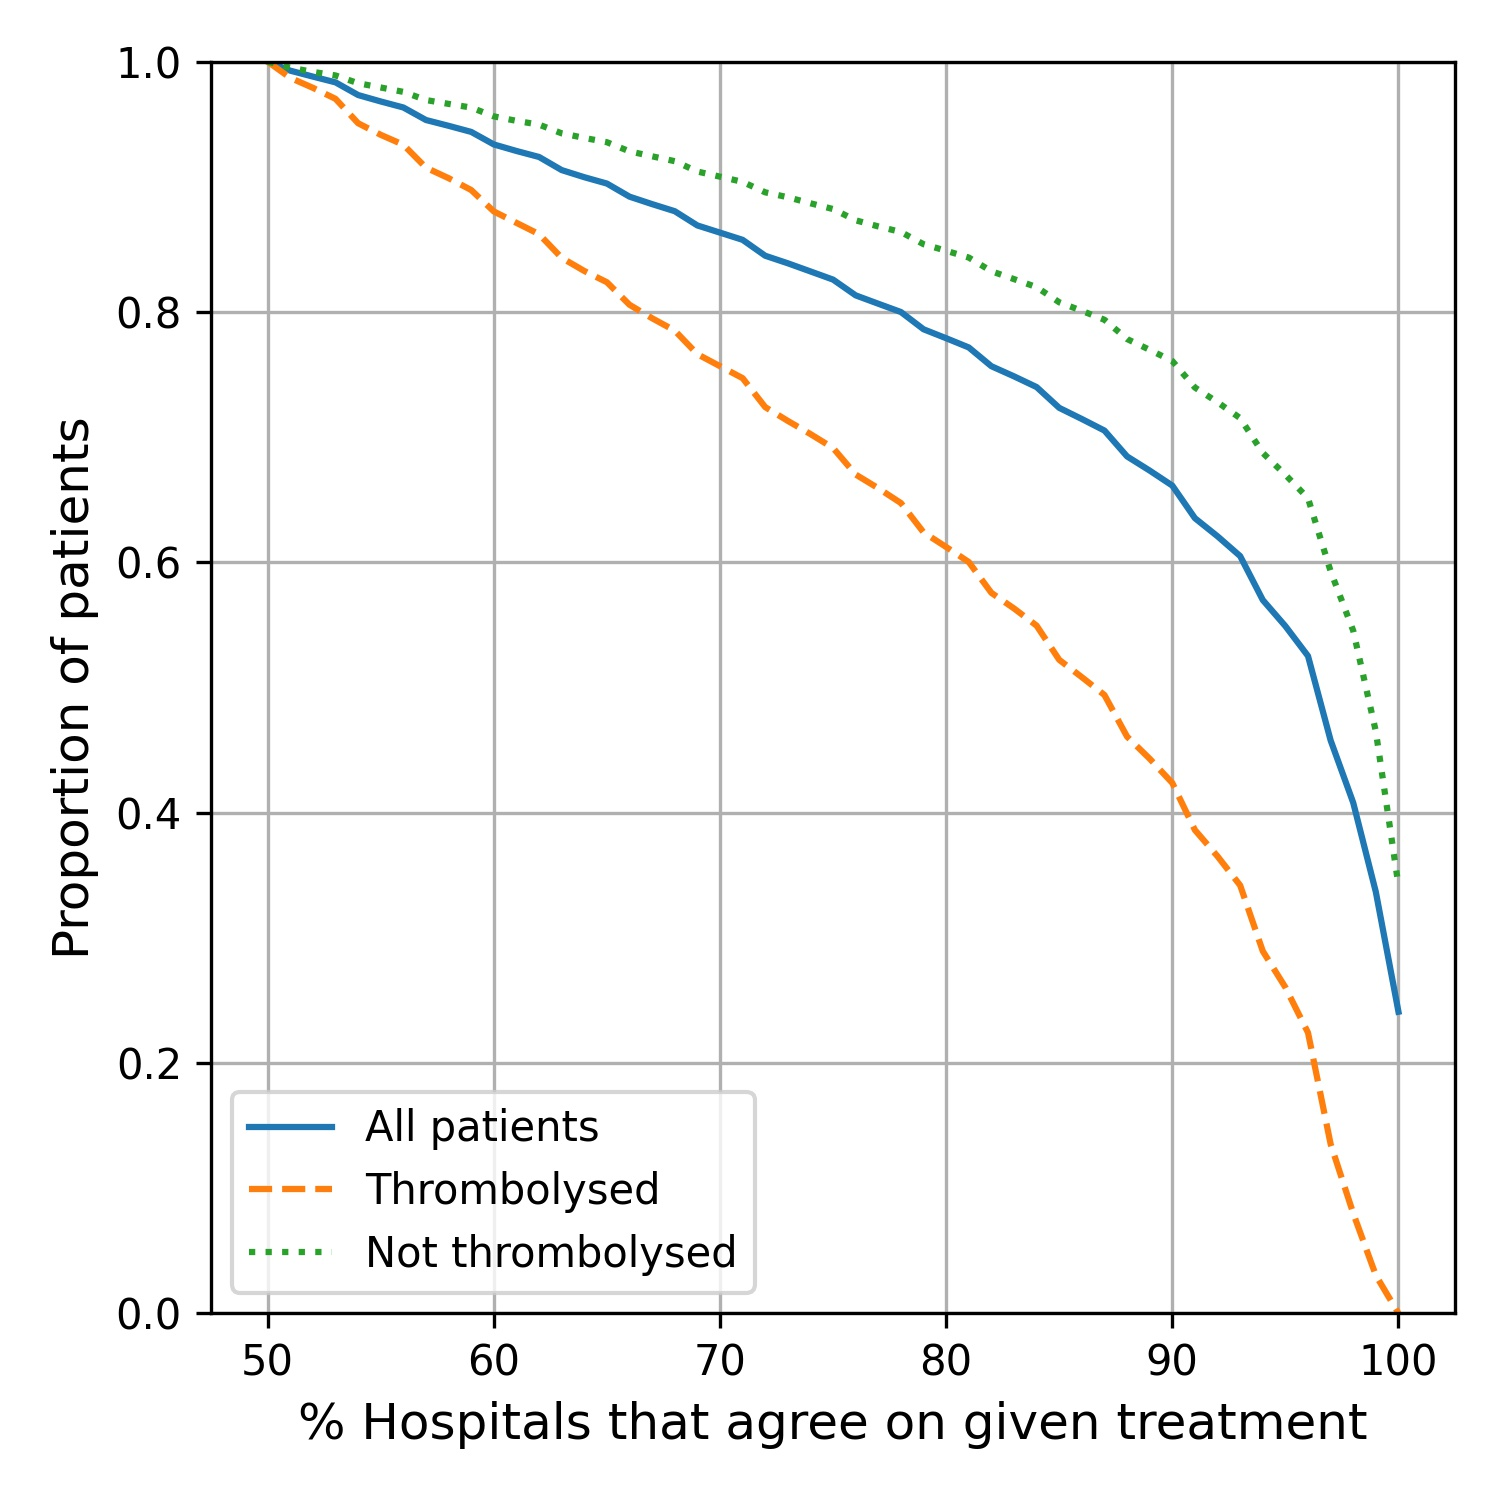
\includegraphics[width=10cm]{figures/agreement_x_hospital_single.jpg}
\caption{Proportion of patients that hospitals agree to treat, stratified by patient outcome.}
\label{fig:aggree}
\end{figure}

\subsection{Grouping hospitals by decision making}

To understand where the variation in decision making occurs, and to group hospitals according to their decision making, we set aside a representative cohort of 10,000 patients and re-trained hospital models on the remaining 78,928 patients. Computing $D_H$ between the predicted outcomes of each pair of hospitals we found no clear groups of hospitals (Figure \ref{fig:cohort_distance_all}), due to the fact that hospitals find it easy to agree on who not to thrombolyse. 

Accounting for this, we re-calculated $D_H$ for each pair of hospitals using only {\it contentious} patients: patients that would have been thrombolysed at 30-70\% of hospitals, of which there were 1,426, reasoning that it is these borderline cases that hospitals with similar decision making processes would make similar decisions on. We found two distinct groups of hospitals (Figure \ref{fig:contentious}). Looking at the thrombolysis rate in contentious patients for each of these groups, the largest group (location 75-95 in Figure \ref{fig:contentious}) has a high thrombolysis rate in this group of patients, with a mean of 90\%, suggesting that these hospitals are more likely to make the decision to thrombolyse when others may consider it risky. 
In contrast, the smaller group in the top left of the figure has a low thrombolysis rate, treating on average 16\% of contentious patients: these are hospitals that are less likely to take risks when the decision to thrombolyse is borderline. 

\begin{figure}[h!]
\centering
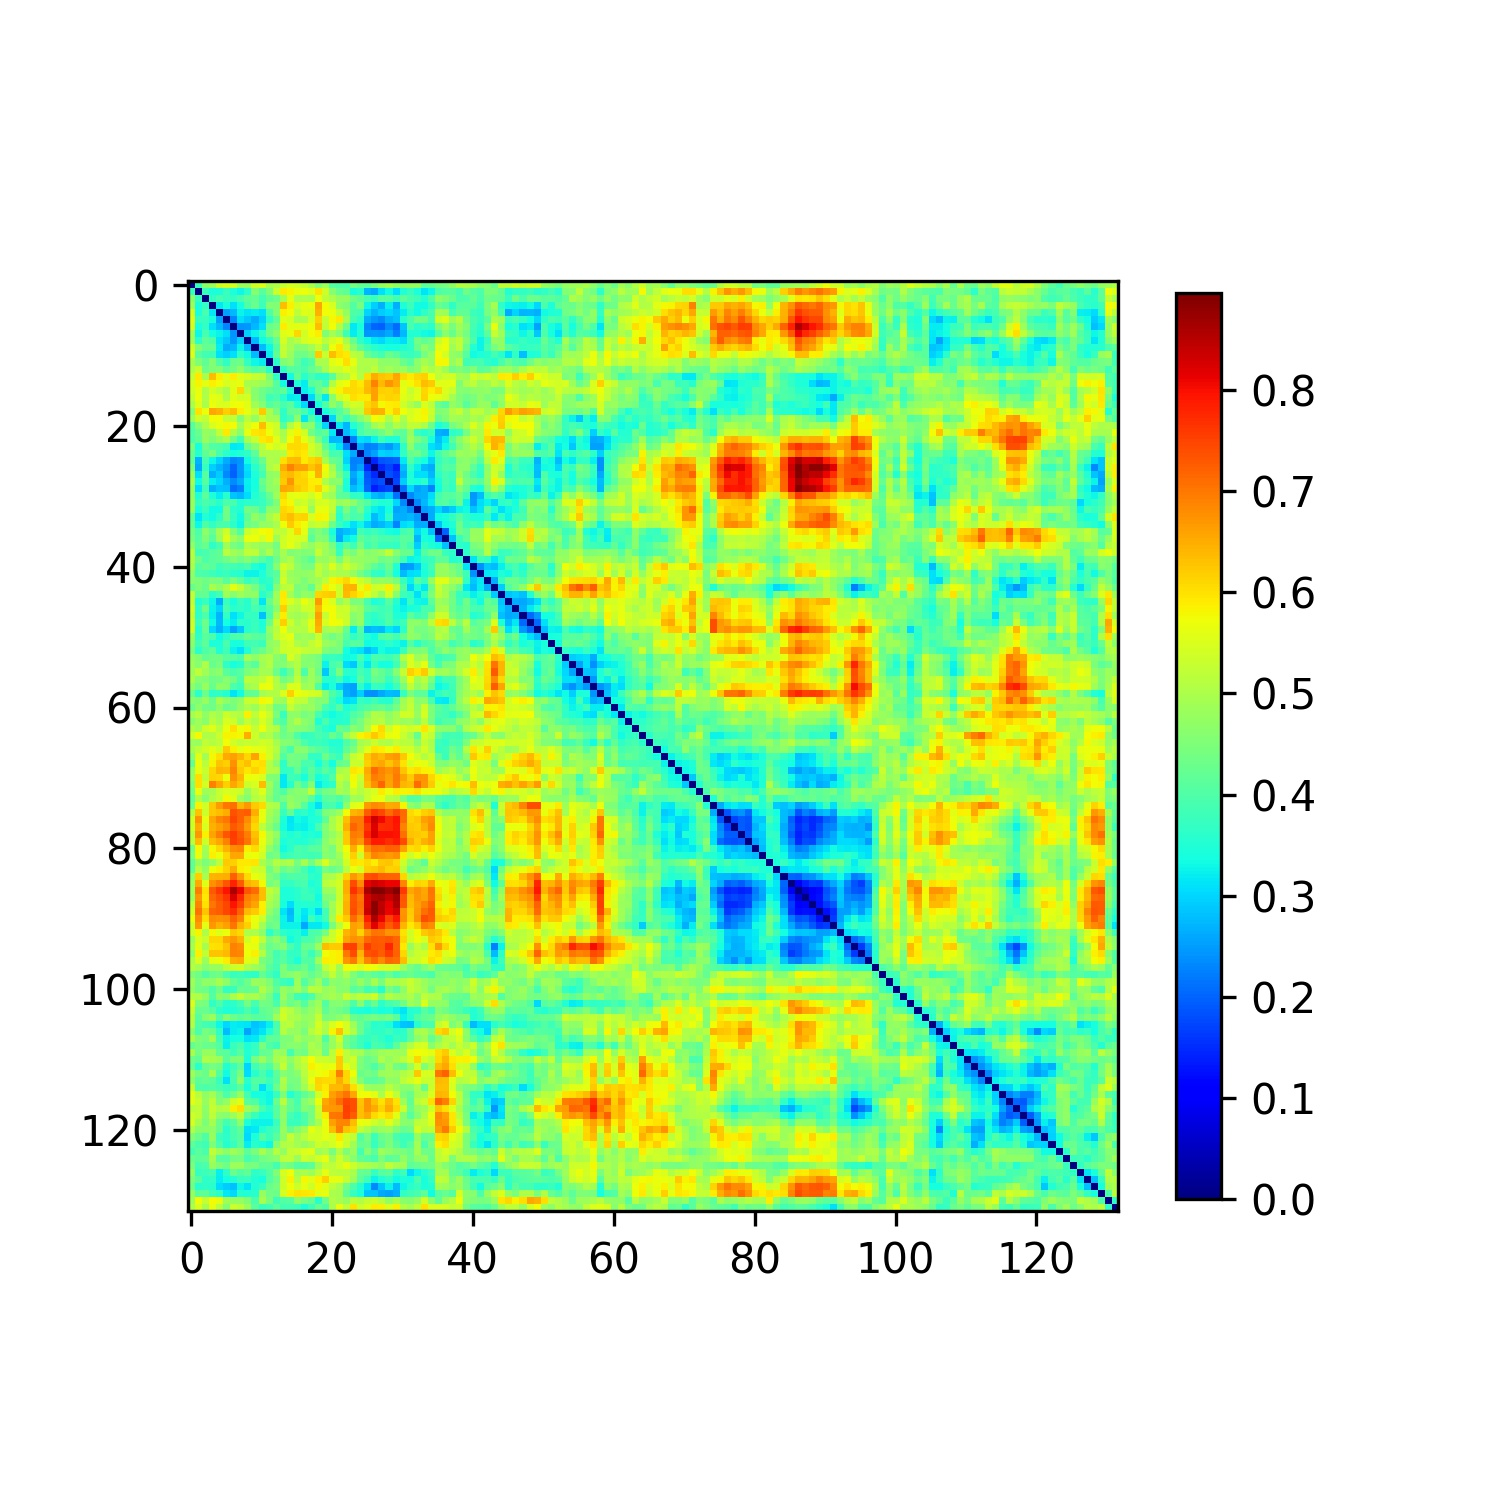
\includegraphics[width=10cm]{figures/cohort_distance.jpg}
\caption{Pairwise Hamming distance, $D_H$, between hospitals, derived from the decisions made at each hospital on how to treat a standardised cohort of 10,000 patients.}
\label{fig:contentious}
\end{figure}

%------------------------ TABLE 3 ------------------------------
    \begin{table}[h]
        \centering
        \begin{tabular}{|l|c|c|c|}
        \hline
        {\bf Measure$^1$} & {\bf Thrombolysed} & {\bf Not Thrombolysed} & {\bf Contentious}  \\
        \hline
        Age & 73 (14) & 76 (14) & 75 (14) \\
        Onset to Arrival & 89 (41) & 123 (55)  & 101 (47) \\
        Arrival to Imaging & 19 (12) & 150 (890)  & 26 (24) \\
        NIHSS & 13 (7) & 6 (7)  & 12 (8) \\
        Rankin before Stroke & 0.6 (1.1)  & 1.2 (1.5) & 1.1 (1.4) \\
        \hline
        \end{tabular}
        \caption{Key measures for patients in a cohort of 10,000 that over 70\% of hospitals would have thrombolysed (Thrombolysed), over 70\% of hospitals wouldn't have thrombolysed (Not Thrombolysed) and those that were contentious (30-70\% of hospitals would have thrombolysed). $^1$Values correspond to mean (std).}
        \label{tab:3}
    \end{table}

%------------------------ TABLE 3 ------------------------------

\subsection{Characterising patients where decision making differs}

We characterized the group of contentious patients by comparing them to patients that were not contentious: patients that over 70\% of hospitals agreed on the treatment of. We found that contentious patients did not differ significantly in terms of age, arrival time, scan time or stroke severity (NIHSS) compared to patients that over 70\% of hospitals would have thrombolysed (Table ~\ref{tab:3}). However there was a difference in terms of disability: the modified rankin score of contentious patients was 1.1 $\pm$ 1.4 where as for those patients that hospitals agreed to thrombolyse, this was 0.6 $\pm$ 1.1, and for patients hospitals agreed not to thrombolyse it was 1.2 $\pm$ 1.5. This suggests patients who have a prior disability represent borderline decisions in terms of whether or not thrombolysis should be given, and more severe disability reduces the chance of thrombolysis. 


To further understand the difference between contentious patients and those that over 70\% of hospitals would have thrombolysed, we trained an additional RF to classify patients into these groups. The RF again performs a binary classification task to determine whether a patient would have been thrombolysed (class 0) or was contentious (class 1). The performance of the RF is a measure of how easy it is to distinguish between these two groups of patients, and determining which features are important for the classification provides insight into how these groups of patients differ. 

\begin{figure}[ht!!!]
\centering
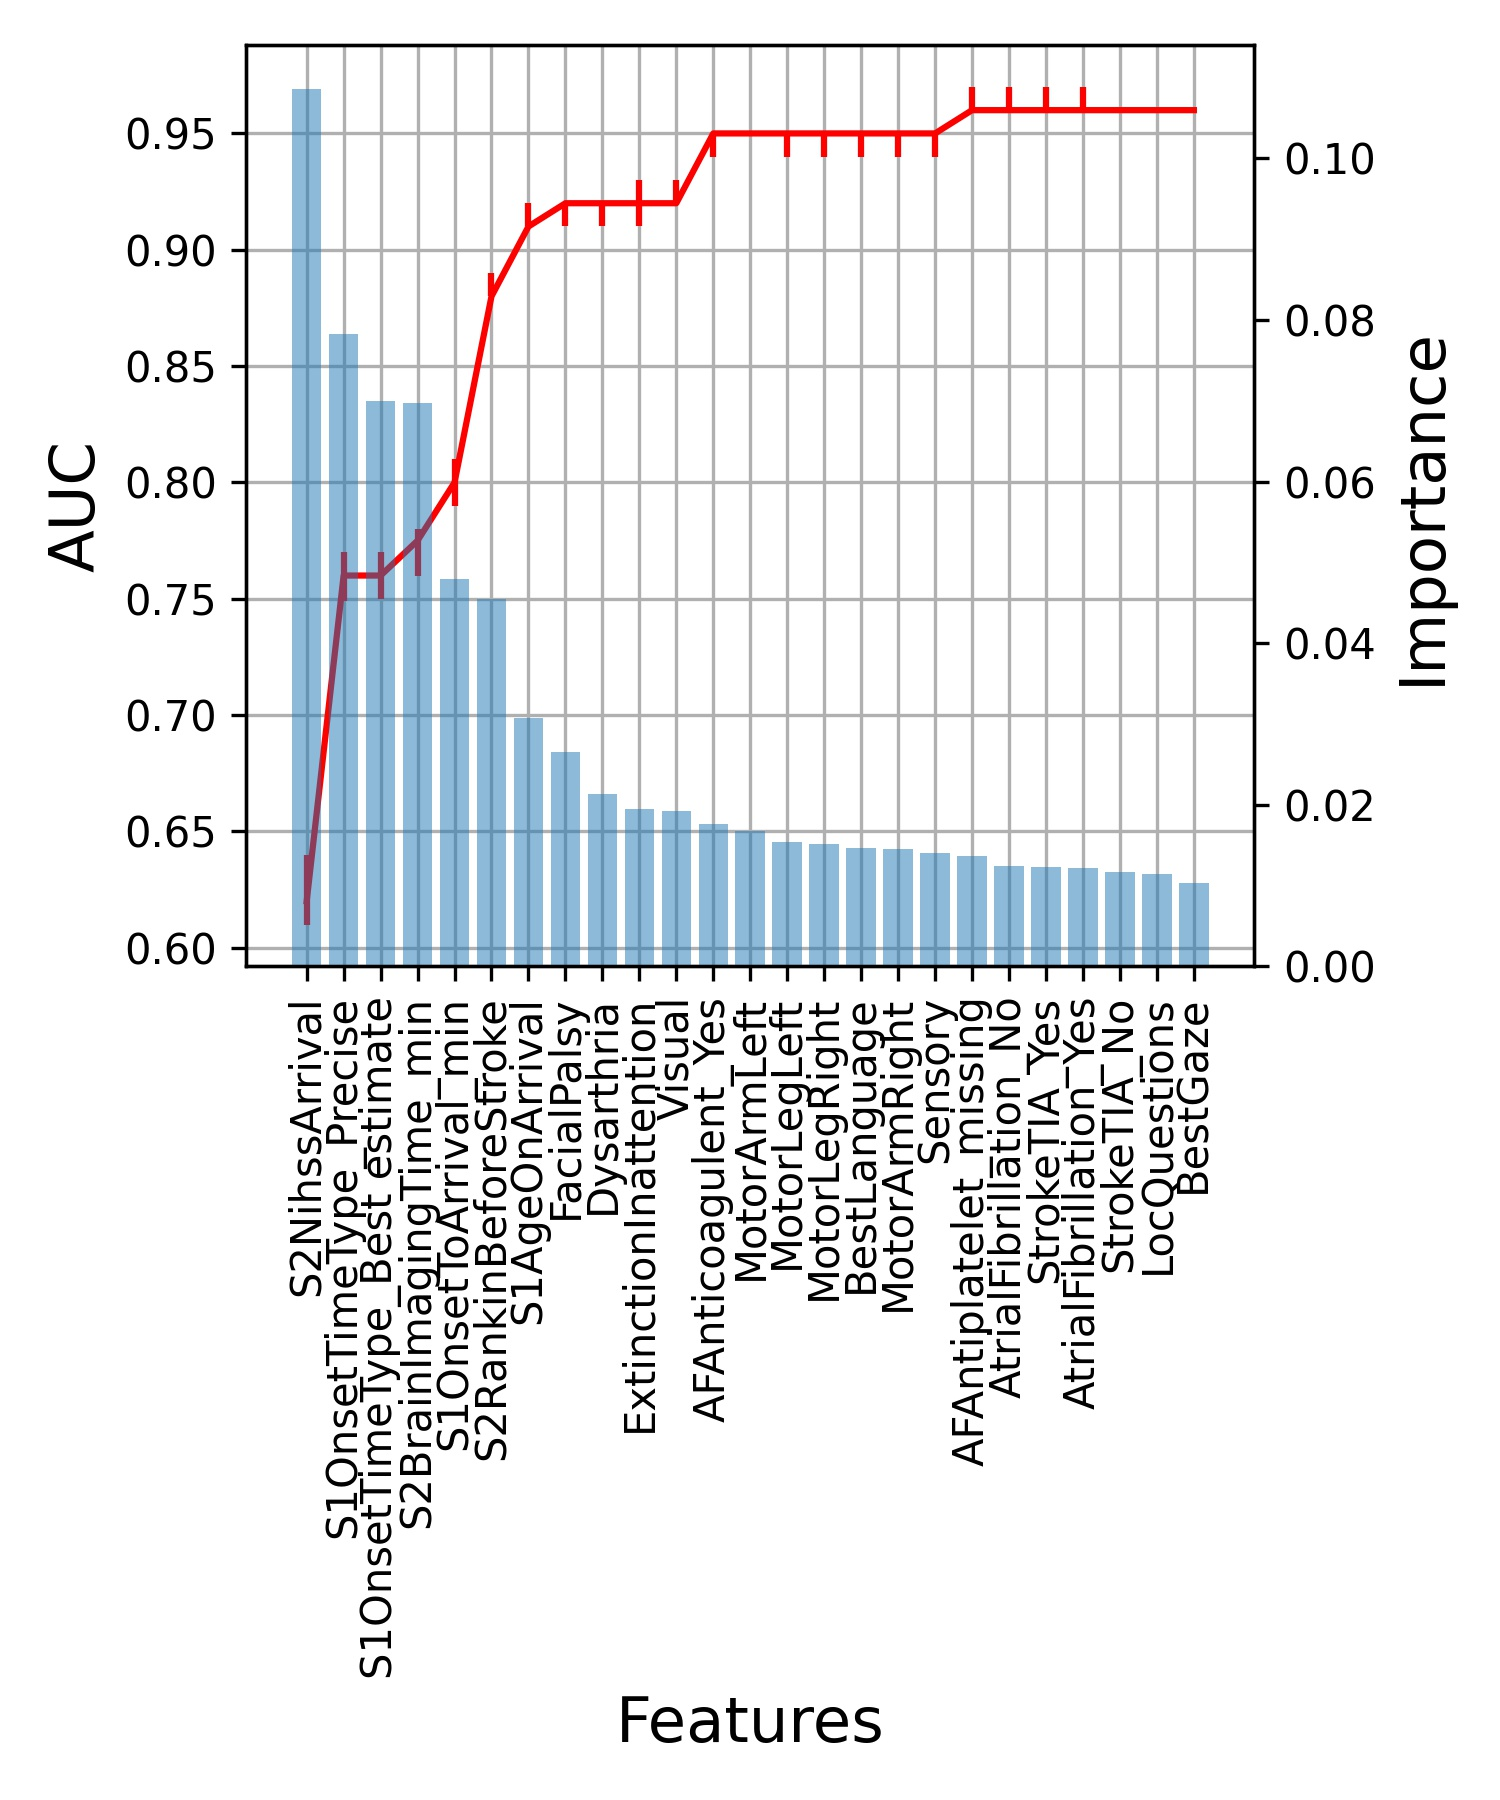
\includegraphics[width=15cm]{figures/auc_features.jpg}
\caption{Features, ordered by importance (x-axis) vs importance (y-axis right) and cumulative AUC (y-axis left) for a random forest trained to classify whether hospitals would agree to thrombolyse a patient or whether they are contentious. Red line represents the median AUC and error bars correspond to 10th and 90th percentiles after bootstrapping the training data 100 times.}
\label{fig:auc_features}
\end{figure}

\begin{figure}[h!!!!]
\centering
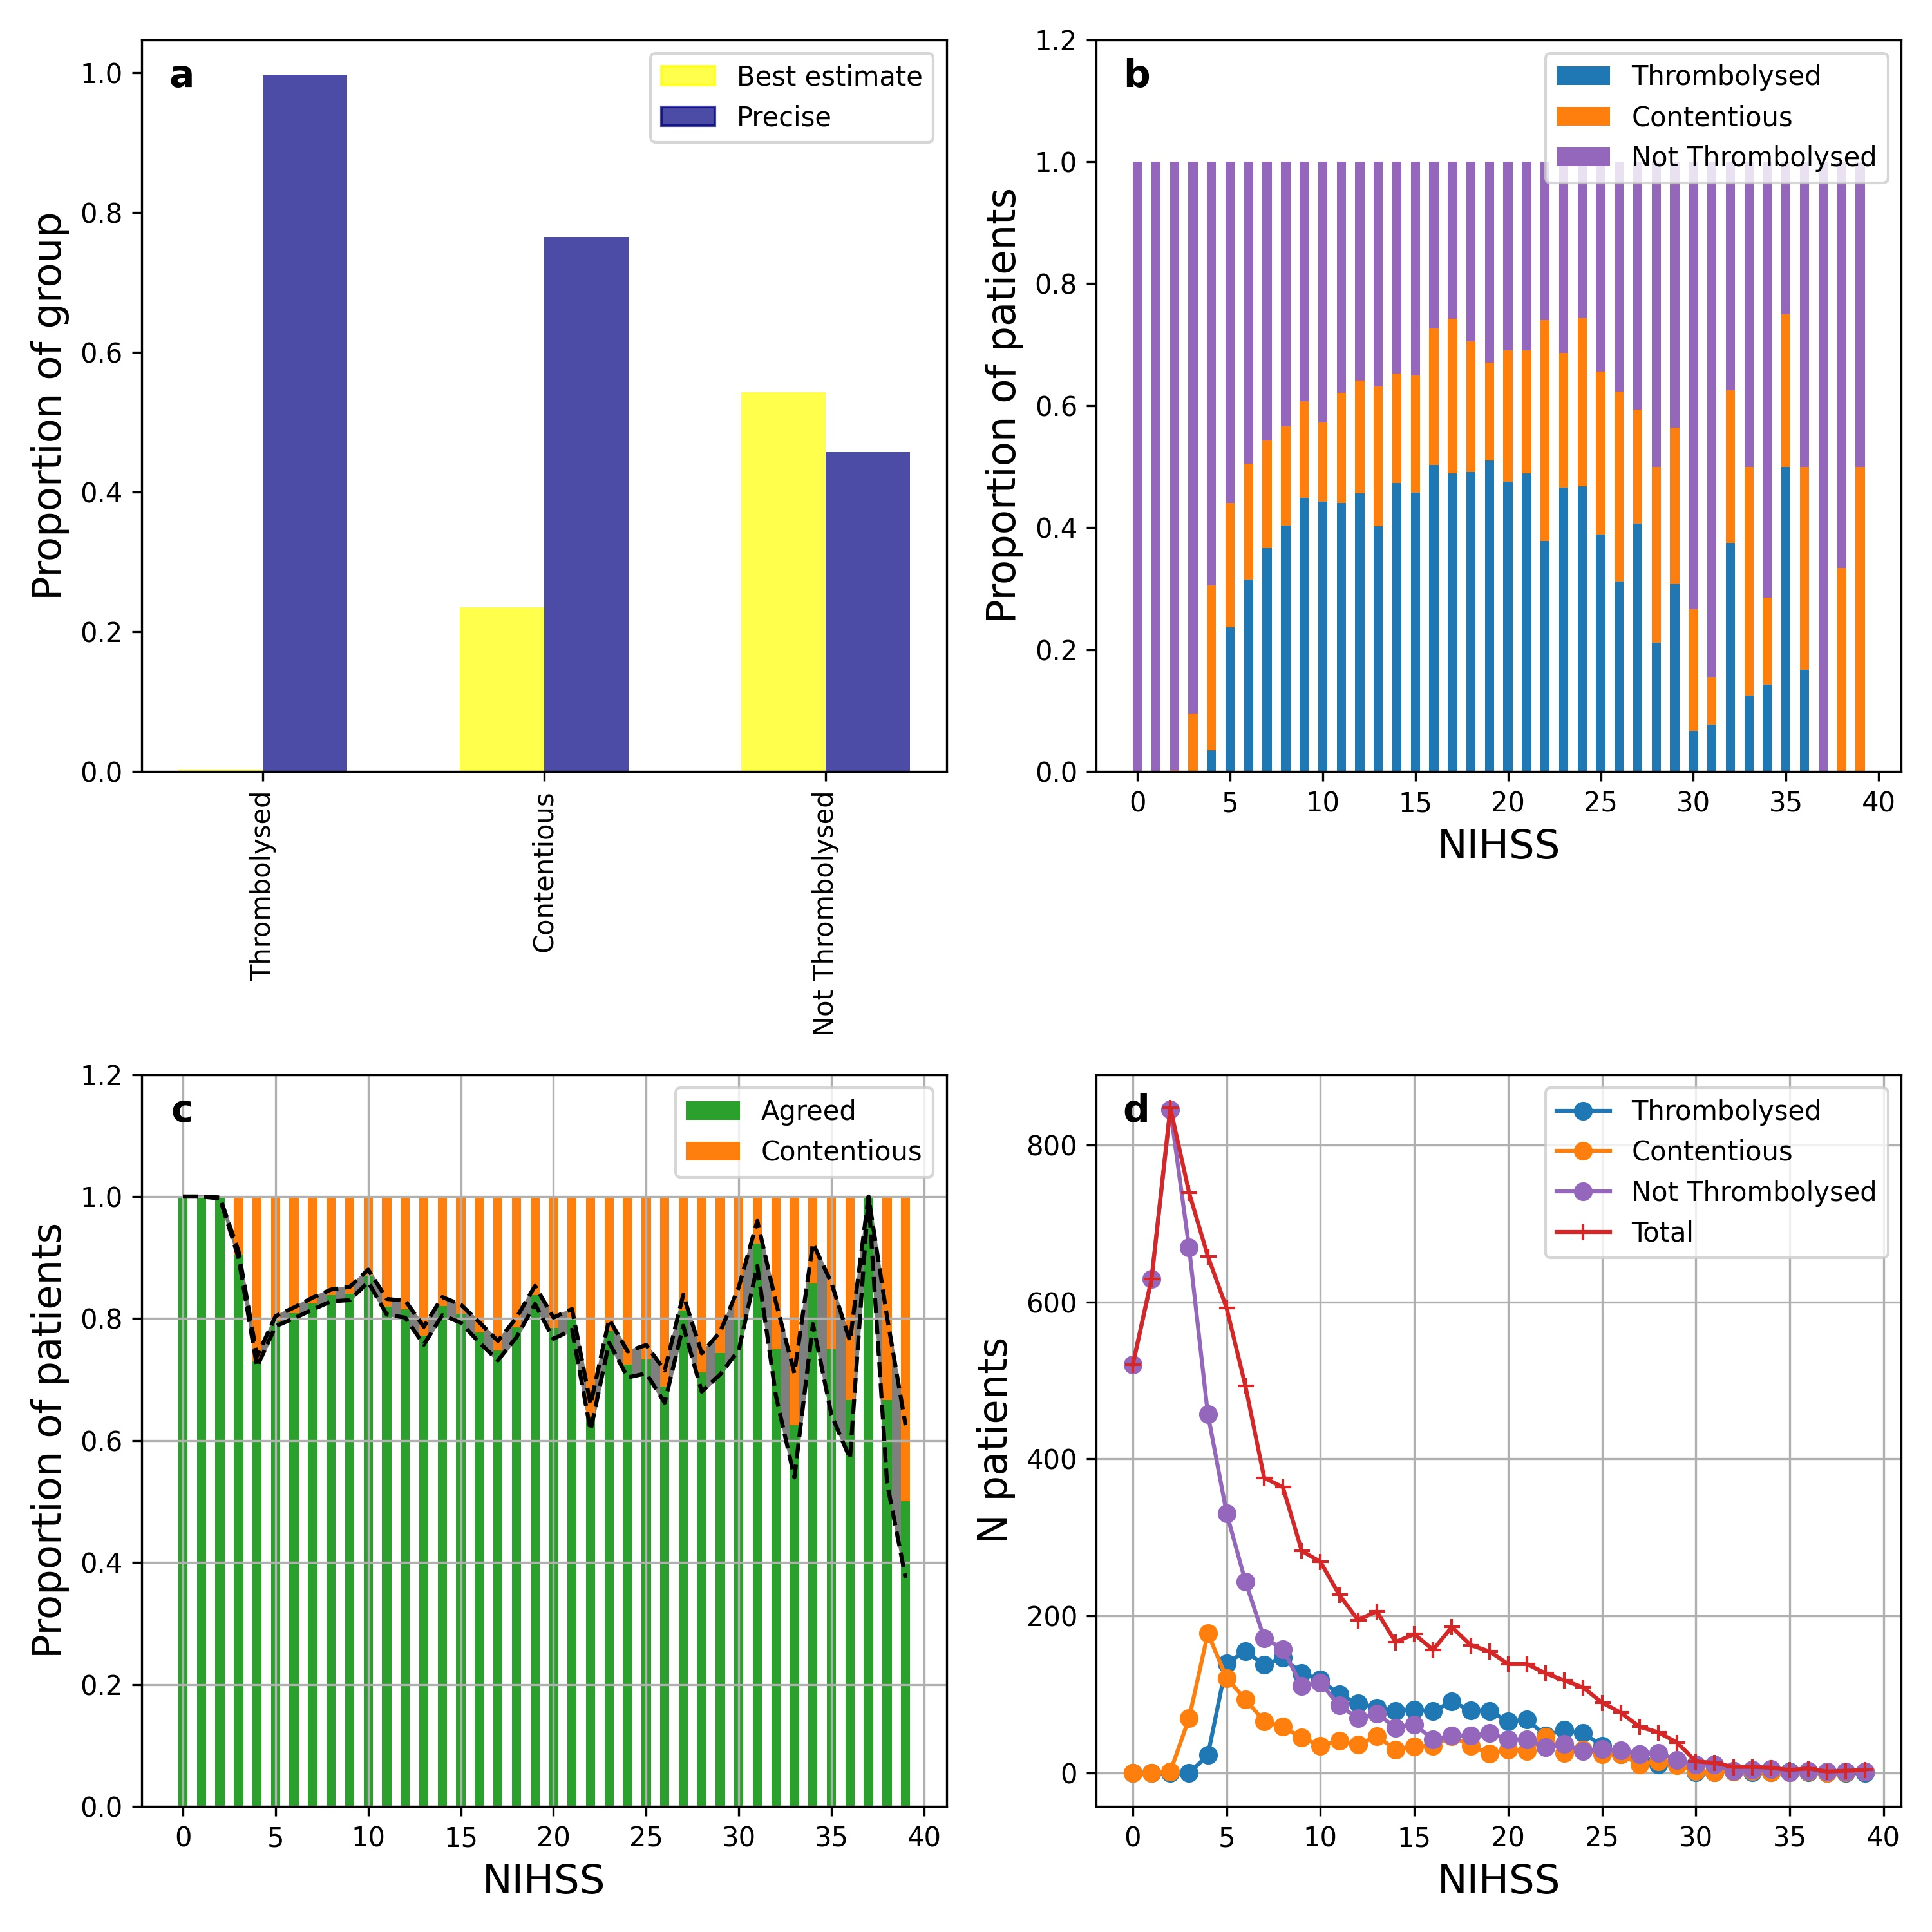
\includegraphics[width=15cm]{figures/nihss_4.jpg}
\caption{{\bf a} Distribution of onset time types for patients in a cohort of 10,000 that over 70\% of hospitals would have thrombolysed (Thrombolysed), patients that over 70\% of hospitals wouldn't have thrombolysed (Not Thrombolysed) and contentious patients. {\bf b} Distribution of NIHSS values for patients in a cohort of 10,000 that over 70\% of hospitals would have thrombolysed (Thrombolysed, blue), over 70\% of hospitals wouldn't have thrombolysed (Not Thrombolysed, purple) and contentious patients (orange). {\bf c} Distribution of NIHSS values for patients that over 70\% of hospitals agreed on how to treat (Agreed, green) and contentious patients (orange). {\bf d} Distribution of NIHSS values for patients in a cohort of 10,000 (Total, red) and stratified by whether over 70\% of hospitals would have thrombolysed (Thrombolysed, blue),  over 70\% of hospitals wouldn't have thrombolysed (Not Thrombolysed, purple) and contentious patients (orange).}
\label{fig:nihss_4}
\end{figure}

The RF was able to classify patients with an accuracy of 88\% (decision threshold of 0.5) and an AUC of 0.96, suggesting that contentious patients are distinguishable from those that 70\% of hospitals would have thrombolysed. To understand how these patients differ, we performed a principal component analysis by re-training the RF with an increasing number of features, starting with the most important. We found that the AUC of the classifier reaches 0.96 with less than 20 features (Figure \ref{fig:auc_features}). Of these features, the most important are NIHSS on arrival and whether the stroke onset time is known or an estimate. 
From Figure \ref{fig:nihss_4}a it is clear that patients that are contentious are more likely to have an estimated onset time than those that hospitals agree to thrombolyse. Figure \ref{fig:nihss_4}b shows, for each NIHSS score, the proportion of patients in each group. Here it is clear that hospitals agree not to thrombolyse patients with very mild stroke, where as contentious patients have moderate to severe stroke (NIHSS 5-30). This pattern is also clear from Figure \ref{fig:nihss_4}c, where we compare the proportion of patients that hospitals agree how to treat (thrombolyse or not thrombolyse), to the contentious group for each NIHSS score. The number of patients with NIHSS $>$ 30, the number of patients is very low (Figure \ref{fig:nihss_4}d) therefore the distributions in Figures \ref{fig:nihss_4}b and c at higher NIHSS values are less representative of the true distribution, as shown by the larger margin of uncertainty in Figure \ref{fig:nihss_4}c. 

For the RF, feature importance is determined by the Gini importance: for each tree a feature’s importance is the total decrease in impurity that occurs when the feature is used to split a node, weighted by the number of samples the node splits. The Gini importance is calculated for each tree and then averaged to give a final feature importance.  Shapley values are an alternative method for determining how each feature contributes to a classification. While Gini importance gives an overall measure of importance for each feature, Shapley values contain information on how the value of a feature contributes to the classifier's final decision. Computing Shapley values themselves is computationally intense, however SHAP (SHapley Additive exPlanations)~\cite{NIPS2017_7062} values provide an estimation of Shapley values and can be used to explain how features contribute to model predictions.

\begin{figure}[ht!!]
\centering
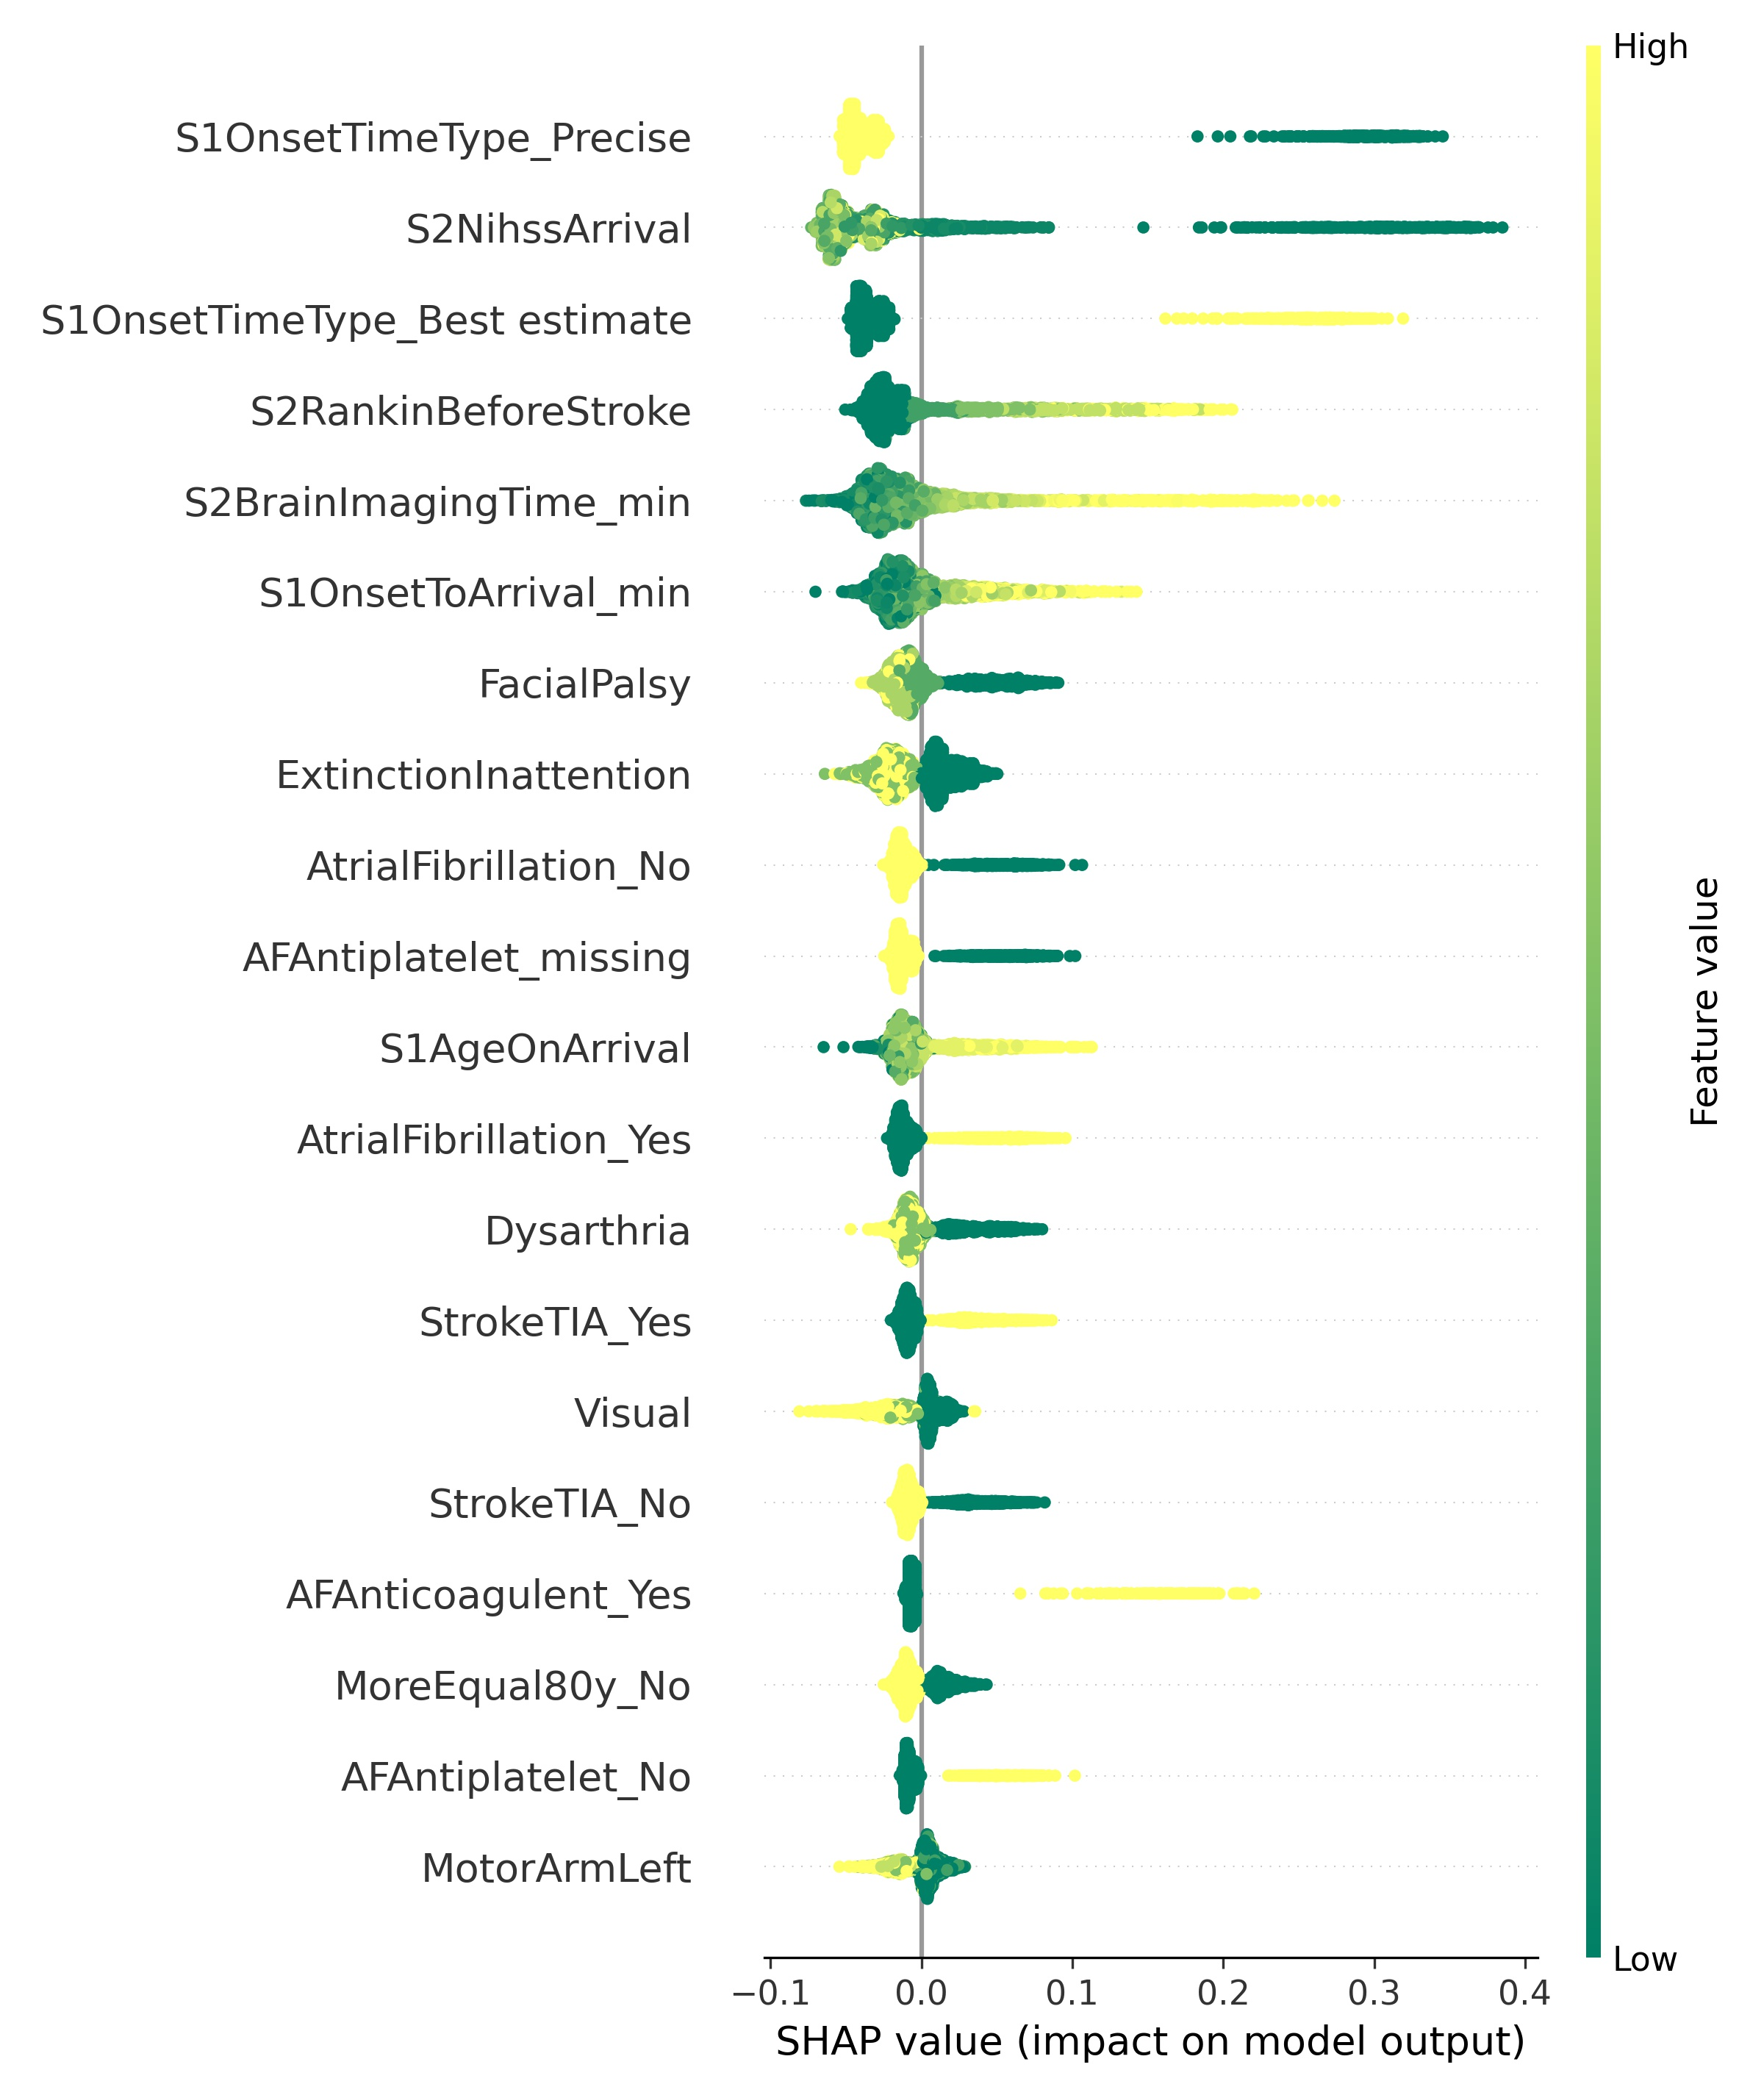
\includegraphics[width=12cm]{figures/shap_beeswarm.jpg}
\caption{SHAP summary plot for a random forest trained to classify whether a patient would have been thrombolysed at over 70\% of hospitals (class 0) or is contentious (class 1).}
\label{fig:shap_beeswarm}
\end{figure}

Figure \ref{fig:shap_beeswarm} displays the SHAP values for the 20 features that have the highest impact on the output of the RF trained to distinguish between patients that hospitals agree to thrombolyse and those that are contentious. For each feature on the y-axis, each point represents the SHAP value of that feature for a single patient. The SHAP value itself (x-axis) tells us whether the feature pushed the model towards classifying a patient as contentious (class 1, positive SHAP) or not (class 0, negative SHAP). For example, from Figure \ref{fig:shap_beeswarm} the most important feature in determining whether a patient would be thrombolysed, or is contentious, is whether or not the onset time is precise. This is a binary feature, where a low value (ie, 0) has a positive SHAP value, corresponding to the onset time being uncertain and pushing a patient towards the contentious class. In contrast, a high value (ie, 1) represents onset time being precisely known and the corresponding SHAP value is negative, pushing a patient towards the class that over 70\% of hospitals would have thrombolysed.

\section{Discussion}

Our methods demonstrate how ML can be used alongside clinical registry data for retrospective audit of decision making. Specifically we have demonstrated that ML can be used to group hospitals according to their decision making and characterise patients that would have been treated differently had they attended a different hospital. 

In our example we have used SSNAP, a clinical registry of in-hospital stroke care in the United Kingdom, to investigate variation in thrombolysis use for acute ischemic stroke in patients having a stroke out of hospital. By training separate RFs on patients from each of 132 hospitals, we found the RFs performed well on their own patients (mean accuracy 84.5\%, mean AUC 0.90). Using these RFs, we assessed the amount of agreement between hospitals by putting all patients through all models, and we found that hospitals were much more likely to agree on the patients not to thrombolyse than those to thrombolyse. Defining contentious patients as those in which there is less agreement between hospitals in how to treat (30-70\% of hospitals would have thrombolysed), we trained an additional RF to discriminate between contentious patients and patients that over 70\% of hospitals would have thrombolysed. We found that contentious patients are principally characterized by uncertainty in time of stroke onset (and therefore time since stroke), milder strokes (as measured by the NIHSS) and higher levels of prior disability (as measured by the mRS). 

In the United Kingdom the current rate of thrombolysis use is 11.1\% of all stroke, which is lower than the target in the NHS Long Term Plan of 20\% and there is significant variation between hospitals (0-24.5\%).  This proportion is also significantly lower than rates reported from large registries in other European countries~\cite{kuhrij2018dutch}, which suggests that there are significant numbers of stroke patients in the UK who stand to benefit from thrombolysis but who are not being treated. The median proportion of patients in whom the time of stroke onset is precisely known is 31.9\%, and in whom it is a ‘best estimate’ is 36.8\%, with 31.4\% classified with an unknown time of onset (SSNAP Annual Results Portfolio, 2020-21 www.strokeaudit.org). However, there is a remarkable variation between hospitals in these proportions, ranging from  0.4-73.3\% in our three-year national sample, a degree of variation that is difficult to understand.  The willingness of individual clinicians to estimate the time of onset may relate to their own perception of the balance of risk and benefit from thrombolysis, particularly among patients at either end of the scale of neurological severity and in those with a greater degree of pre-stroke disability.  
%
A previous study~\cite{de2018factors} investigated factors that influence variation in thrombolysis decision-making using a discrete choice experiment involving 138 clinicians, who were presented with hypothetical vignettes and asked how they would treat the patients described. This study also found that stroke severity and pre-stroke disability influenced a clinician’s decision of whether or not to thrombolyse a patient. More recent imaging methods for acute stroke, using CT perfusion or MRI techniques, now offer the prospect of identifying patients eligible for thrombolysis according to a ‘tissue window’ as opposed to the more widely used ‘time window’~\cite{thomalla2020intravenous}. These developments would permit a more objective assessment of the ‘tissue at risk’ as the justification for thrombolysis at any time point after onset (known or unknown), and may enable clinical decision-making to become less variably based on individual clinicians’ judgements about the accuracy of onset times or pre-stroke disabilities.  Moving towards greater objectivity in deciding eligibility for thrombolysis may reduce the significant and unexplained variation in practice that we have highlighted in this study, which persists over more than 25 years since the first publication of the evidence for thrombolysis in acute ischemic stroke~\cite{tissue1995national}. Identifying and characterizing the types of patients in whom eligibility is contentious also suggests areas where further clinical research is appropriate, and may help to improve the training of clinical decision-makers in thrombolysis, and thereby increase the consistency in thrombolysis use in the future. 
%
 

\subsection{Study Limitations}

When investigating the calibration of the hospital models we found that hospitals with both lower thrombolysis rates and fewer patients than average had less well calibrated models. This highlights the fact that when using an ML approach its important to consider whether there is both a sufficient amount of data in total (number of patients) and sufficient data in each class (thrombolysis rate) for the algorithms to perform well. 

Performance of ML algorithms is also dependent on the level of detail contained in the data being used. We have demonstrated that hospital models perform well on their own patients, however it is likely that there are parameters that are not measured in SSNAP which are also significant contributors to variation in thrombolysis practice. It is therefore possible that parameters not present in the data, such as organizational factors like the availability and proximity of a CT scanner, or the availability of a stroke physician, impact model performance.

Our predictions about differences in clinical decision-making are necessarily at site level. We pick up on general differences in attitude to thrombolysis between sites, but we cannot detect differences that exist between individual clinicians (as decision-making is the end-result of a process, and may be collective, it may be that decisions can never be fully assigned to an individual).

In the example presented we used random forest algorithms due to their robustness, and previous work~\cite{samuelbook} has shown that, for this specific example, RF performs comparably to a neural network, and is superior to a logistic regression. However, the methods we have presented are more general and can be used alongside any ML algorithm. 




\section{Conclusion}

The use of machine learning as applied to large-scale national stroke registry data can improve our understanding of the sources of variation in decision-making between hospitals in critical areas of clinical practice such as thrombolysis in acute ischemic stroke. The learning derived from advanced analysis could be used to reduce clinical variation through more effective audit and feedback to participating sites, and increase both the consistency of decision-making and the overall use and population benefit from treatments. The wider adoption of machine learning techniques in other comprehensive clinical registries similarly offers the prospect of reducing clinical variation in many other important disease areas.

\section*{Acknowledgments}

We would like to thank the SAMueL project team (Julia Frost, Kristin Liabo, Kerry Pearn, Tom Monks, Zhivko Zhelev, Stuart Logan, Ken Stein, Leon Farmer, Penny Thompson) for their input into this work.

\subsection*{Funding}

This report is independent research funded by the National Institute for Health Research Applied Research Collaboration South West Peninsula and by the National Institute for Health Research Health and Social Care Delivery Research (HSDR) Programme [HS\&DR 17/99/89]. The views expressed in this publication are those of the authors and not necessarily those of the National Institute for Health Research or the Department of Health and Social Care.

\subsection*{Conflict of interest statement}

All authors declare no conflicts of interest.

\bibliographystyle{unsrt}
\bibliography{samuel}



\clearpage

%------------------------ SUPPLEMENTARY MATERIAL ------------------

\beginsupplement
\section*{Supplementary Information}

%------------------------ TABLE S1 ------------------------------

   % \begin{table}[h!]
    %    \centering
        \begin{longtable}{|l|p{8.5cm}|c|}
        \hline
        {\bf Feature} & {\bf Description} & {\bf Category} \\
        \hline
        \endhead
        \hline
        \endfoot
        \endlastfoot
        Stroke Team & Pseudonymised SSNAP team unique identifier & Categorical \\
        Pathway & Episode number. Refers to the patient's pathway (i.e. team transfers) & Ordinal \\
        Age & Age on arrival aggregated to 5 year bands & Discrete \\
        >= 80 years & Whether the patient is >= 80 years old at the moment of the stroke & Binary \\
        Gender & Gender & Binary \\
        Ethnicity & Patient Ethnicity. Aggregated to White, Black, Mixed, Asian and Other & Categorical \\
        Onset in hospital & Whether the patient was already an inpatient at the time of stroke & Binary \\
        Onset to arrival (minutes) & Time from symptom onset to arrival at hospital in minutes, where known and if out of hospital stroke & Continuous \\
        Onset Date Type & Whether the date of onset given is precise, best estimate or if the stroke occurred while sleep & Categorical \\
        Onset Time Type & Whether the time of symptom onset given is precise, best estimate, not known & Categorical \\
        Arrive by Ambulance & Whether the patient arrived by ambulance & Binary \\
        Admission Hour & Hour of arrival, aggregated to 3 hour epochs & Categorical \\
        Admission Day & Day of week at the moment of admission & Categorical \\
        Admission Quarter & Year quarter (Q1: Jan-Mar; Q2:April-Jun; Q3: Jul-Sept; Q4: Oct-Dec) & Categorical \\
        Admission Year & Year of admission & Categorical \\
        Congestive Heart Failure &Comorbidbities: Pre-Stroke Congestive Heart Failure  & Binary \\
        Hypertension & Comorbidbities: Pre-Stroke Systemic Hypertension & Binary \\
        Atrial Fibrillation & Comorbidities: Pre-Stroke Atrial Fibrillation (persistent, permanent, or paroxysmal) & Binary \\
        Diabetes & Comorbidities: Pre-Stroke Diabetes Mellitus & Binary \\
        Stroke TIA & Comorbidities: Pre-Stroke history of stroke or Transient Ischaemic Attack (TIA) & Binary \\
        AF Antiplatelet & Only available if "Yes" to Atrial Fibrillation (Q2.1.3). Whether the patient was on antiplatelet medication prior to admission                              & Binary \\
        AF Anticoagulent & Prior to 01-Dec-2017: Only available if "Yes" to Atrial Fibrillation (Q2.1.3); From 01-Dec-2017: available even if patient is not in Atrial Fibrillation prior to admission. Whether the patient was on anticoagulant medication prior to admission & Binary \\
        AF Anticoagulent Vitamin K & If the patient was receiving anticoagulant medication, was it vitamin K antagonists & Binary \\
        AF Anticoagulent DOAC & If the patient was receiving anticoagulant medication, was it direct oral anticoagulants (DOACs) & Binary \\
        AF Anticoagulent Heparin & If the patient was receiving anticoagulant medication, was it Heparin & Binary \\
        New AF Diagnosis & Whether a new diagnosis of Atrial Fibrillation was made on admission & Binary \\
        Rankin Before Stroke & Patient's modified Rankin Scale score before this stroke (Higher values indicate more disability) & Ordinal \\
        Loc & National Institutes of Health Stroke Scale Item 1a Level of Consciousness (higher values indicate more severe deficit) & Ordinal \\
        Loc Questions & National Institutes of Health Stroke Scale Item 1b Level of Consciousness Questions (higher values indicate more severe deficit) & Ordinal \\
        Loc Commands & National Institutes of Health Stroke Scale Item 1c Level of Consciousness Commands (higher values indicate more severe deficit) & Ordinal \\
        Best Gaze & National Institutes of Health Stroke Scale Item 2 Best Gaze (higher values indicate more severe deficit) & Ordinal \\
        Visual & National Institutes of Health Stroke Scale Item 3 Visual Fields (higher values indicate more severe deficit) & Ordinal \\
        Facial Palsy & National Institutes of Health Stroke Scale Item 4 Facial Paresis (higher values indicate more severe deficit) & Ordinal \\
        Motor Arm left & National Institutes of Health Stroke Scale Item 5a Motor Arm - Left (higher values indicate more severe deficit) & Ordinal \\
        Motor Arm right & National Institutes of Health Stroke Scale Item 5b Motor Arm - Right (higher values indicate more severe deficit) & Ordinal \\
        Motor Leg left & National Institutes of Health Stroke Scale Item 6a Motor Leg - Left (higher values indicate more severe deficit) & Ordinal \\
        Motor Leg right & National Institutes of Health Stroke Scale Item 6b Motor Leg - Right (higher values indicate more severe deficit) & Ordinal \\
        Limb Ataxia & National Institutes of Health Stroke Scale Item 7 Limb Ataxia (higher values indicate more severe deficit) & Ordinal \\
        Sensory & National Institutes of Health Stroke Scale Item 8 Sensory (higher values indicate more severe deficit) & Ordinal \\
        Best Language & National Institutes of Health Stroke Scale Item 9 Best Language (higher values indicate more severe deficit) & Ordinal \\
        Dysarthria & National Institutes of Health Stroke Scale Item 10 Dysarthria (higher values indicate more severe deficit) & Ordinal \\
        Extinction Inattention & National Institutes of Health Stroke Scale Item 11 Extinction and Inattention (higher values indicate more severe deficit) & Ordinal \\
        NIHSS Arrival & National Institutes of Health Stroke Scale score on arrival at hospital & Discrete \\
        Brain Imaging Time (minutes) & Time from Clock Start to brain scan. In minutes. "Clock Start" is used throughout SSNAP reporting to refer to the date and time of arrival at first hospital for newly arrived patients, or to the date and time of symptom onset if patient already in hospital at the time of their stroke. & Continuous \\
        Stroke Type & Whether the stroke type was infarction or primary intracerebral haemorrhage & Binary \\
        TIA in last month & Whether the patient had a Transient Ischaemic Attack during the last month. Item from the SSNAP comprehensive dataset questions (not mandatory) & Binary \\
        \hline
        \caption{Features in SSNAP used for training the combined model}
        \label{tab:S1}       
        \end{longtable}

 %   \end{table}

%------------------------ TABLE S1 ------------------------------

%------------------------ TABLE S2 ------------------------------

    \begin{table}[h!]
        \centering
        \begin{tabular}{|l|c|c|}
        \hline
        {\bf Feature} & {\bf \% Missing} & {\bf Imputation method}  \\
        \hline
        AF Antiplatelet & 79.3 & missing \\
        AF Anticoagulent & 50.6 & missing \\
        AF Anticoagulent Vitamin K & 62.5 & missing \\
        AF Anticoagulent DOAC & 62.5 &  missing \\
        AF Anticoagulent Heparin & 62.5 & missing \\
        New AF Diagnosis & 72.0 & missing \\
        Loc Questions & 2.2 &  0 \\
        Loc Commands & 2.1 & 0 \\
        Best Gaze & 2.7 & 0 \\
        Visual & 3.6 &  0 \\
        Facial Palsy & 2.1 & 0 \\
        Motor Arm left & 2.1 & 0 \\
        Motor Arm right & 2.1 & 0 \\
        Motor Leg left & 2.2 & 0 \\
        Motor Leg right & 2.2 & 0 \\
        Limb Ataxia & 4.0 & 0 \\
        Sensory & 3.5 & 0 \\
        Best Language & 2.3 & 0 \\
        Dysarthria & 2.8 & 0 \\
        Extinction Inattention & 2.8 & 0 \\
        NIHSS Arrival & 5.8 & 0 \\
        Brain Imaging Time (minutes) & 0.2 & 9999 \\
        Stroke Type & 0.2 & missing \\
        TIA in last month & 91.0 & missing \\
        
        \hline
        \end{tabular}
        \caption{Amounts of missing data in SSNAP and imputation method used.}
        \label{tab:S2}
    \end{table}

%------------------------ TABLE S2 ------------------------------
\begin{figure}[h]
\centering
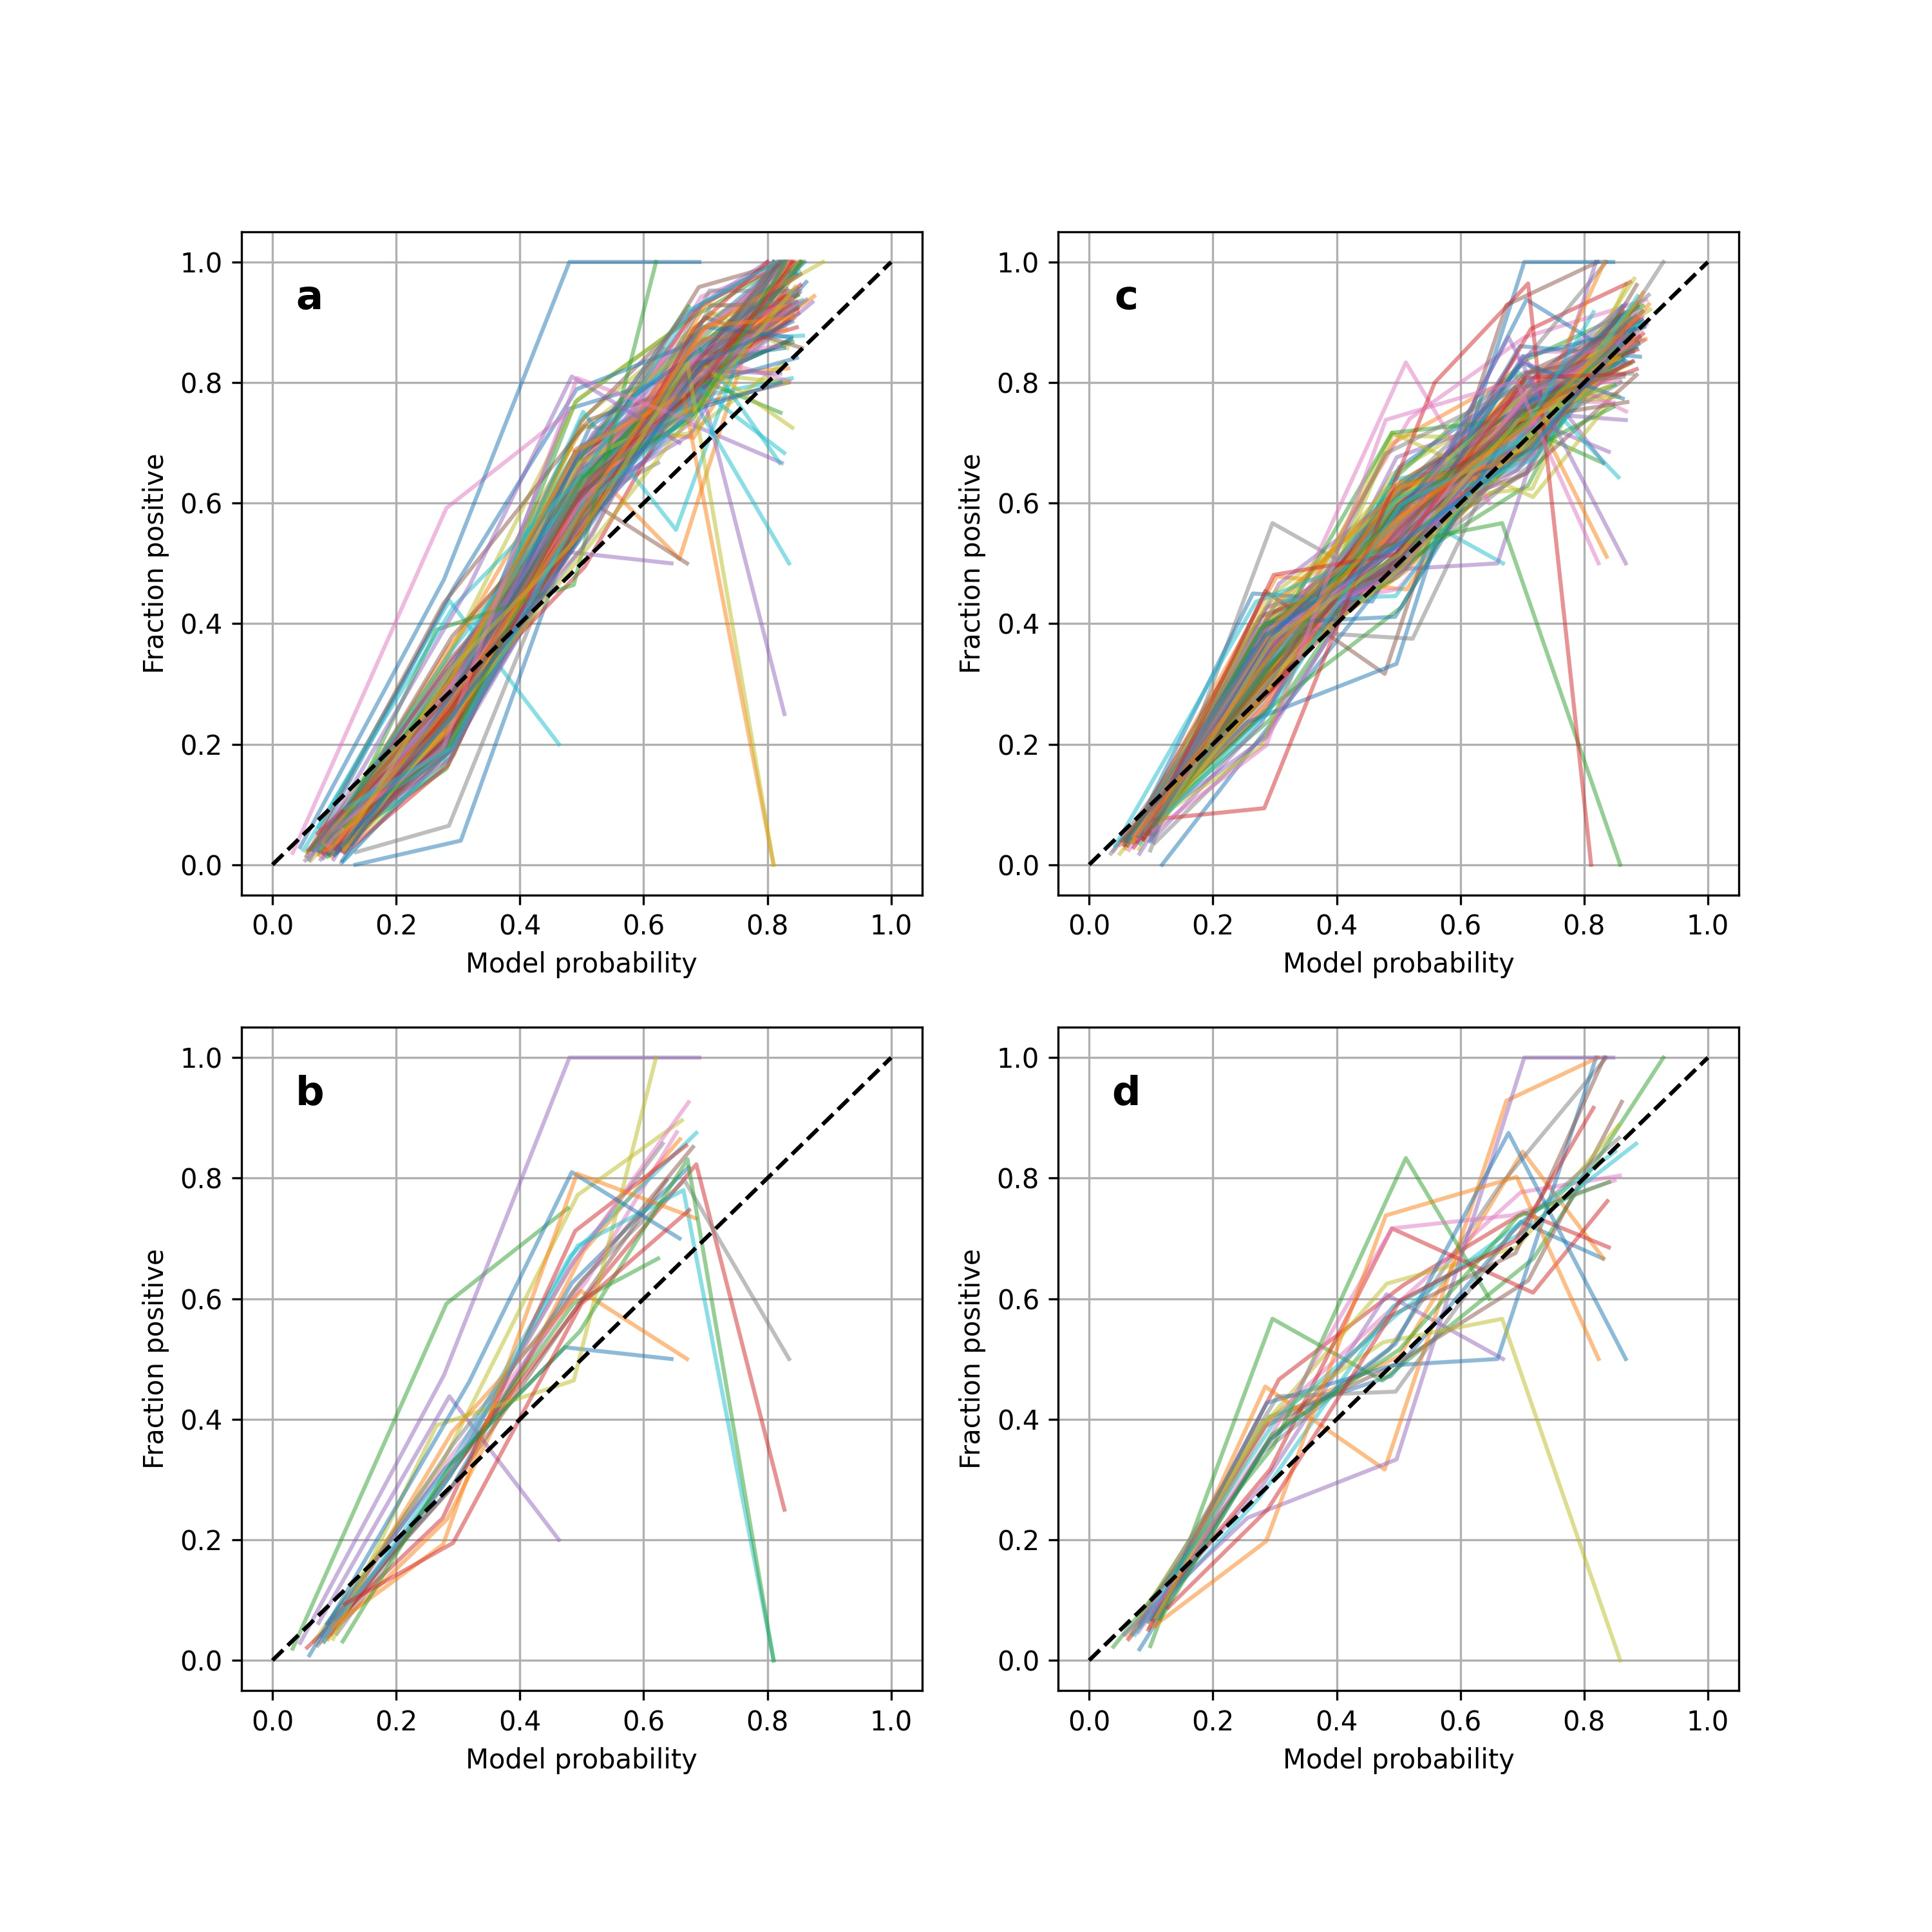
\includegraphics[width=16cm]{figures/calibration_curves_sigmoid.jpg}
\caption{{\bf a} Calibration curves for all hospital models {\bf b} Calibration curves for hospital models that were not well calibrated {\bf c} Calibration curves for all hospital models after applying Platt Scaling {\bf d} Calibration curves for hospitals models that were originally not well calibrated after applying Platt Scaling}
\label{fig:calibration}
\end{figure}

\begin{figure}[h]
\centering
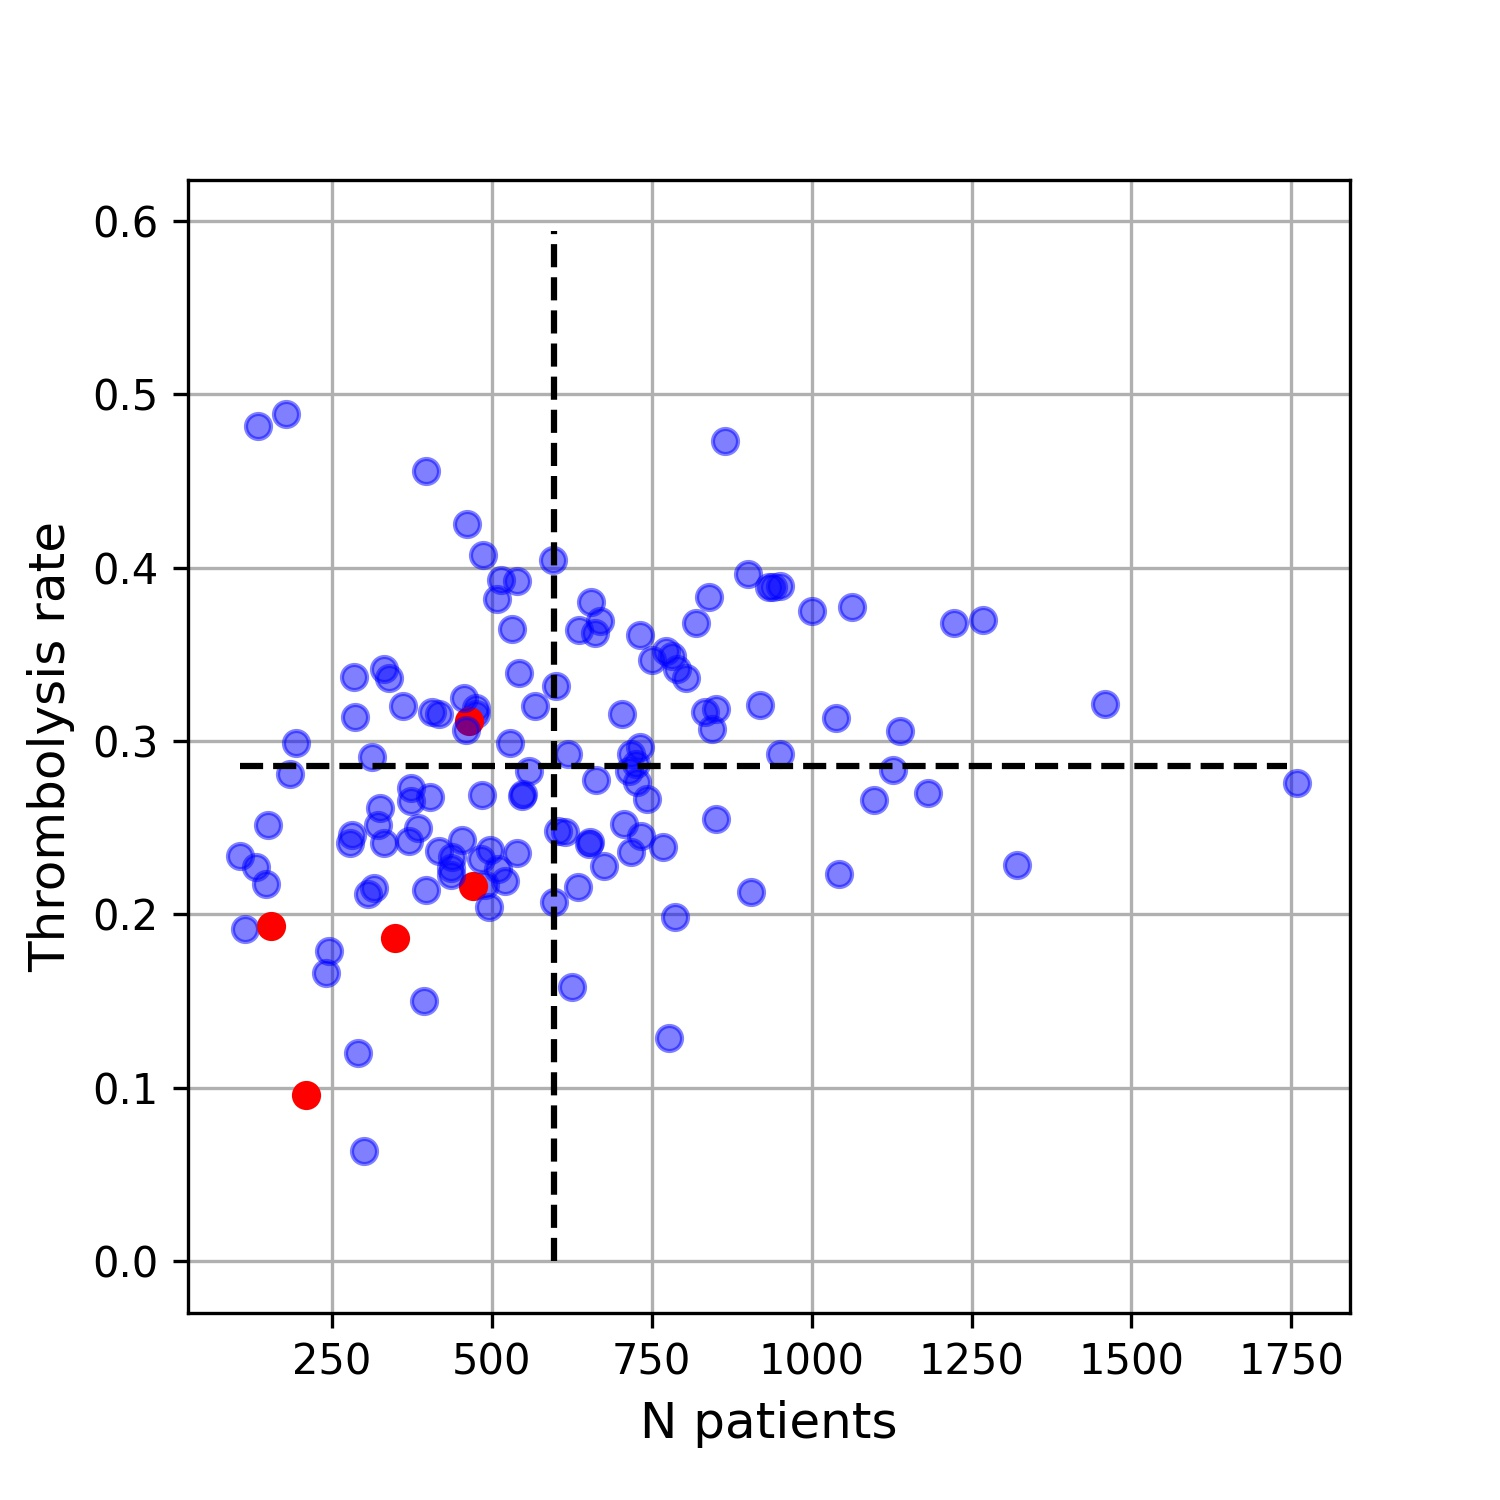
\includegraphics[width=10cm]{figures/uncalibrated.jpg}
\caption{Number of patients (x-axis) vs thrombolysis rate (y-axis) for hospitals that were well calibrated (blue) and those that were not well calibrated (red). Black dashed lines represent mean values along each axis.}
\label{fig:uncalibrated}
\end{figure}


\begin{figure}[h]
\centering
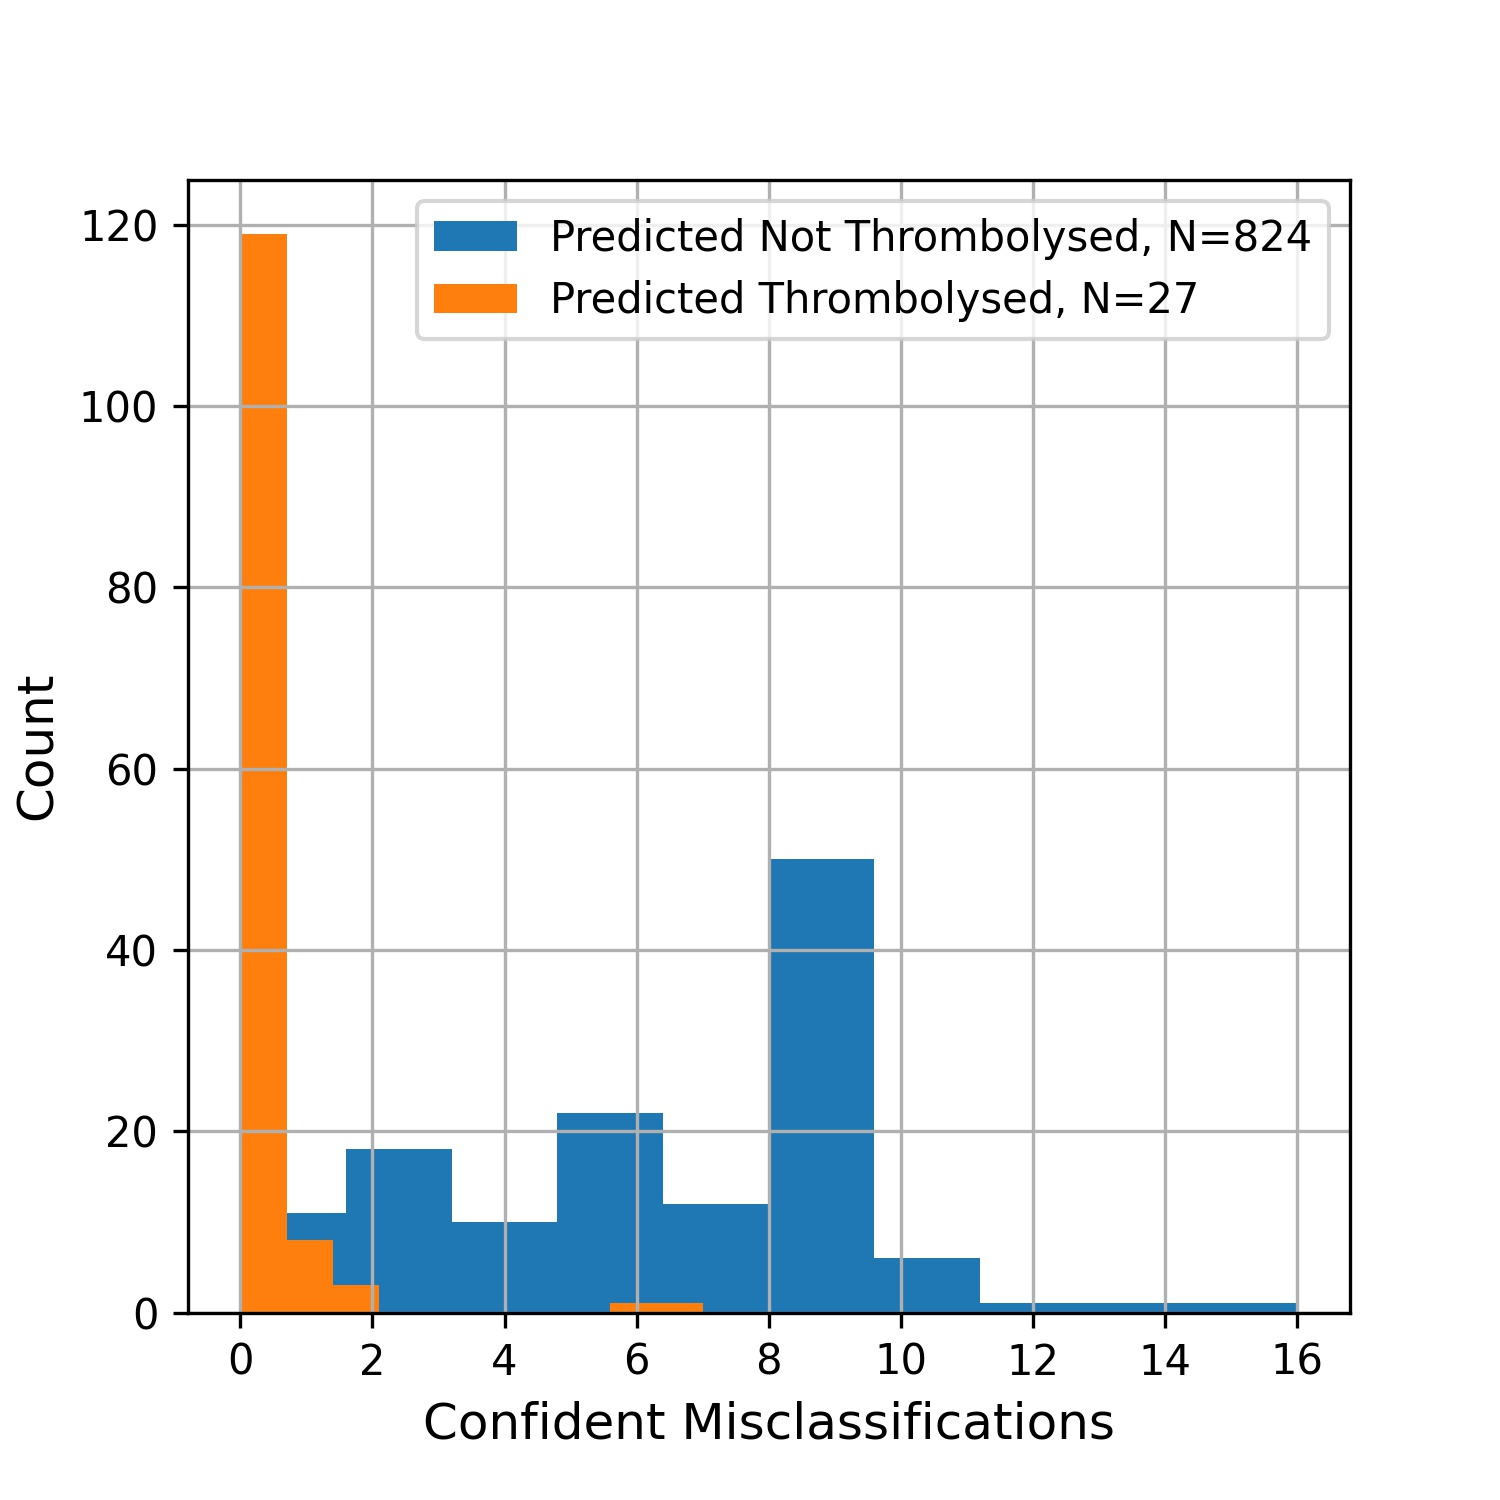
\includegraphics[width=10cm]{figures/missclassified_histogram.jpg}
\caption{Histogram of confident misclassifications for hospital models, stratified by model outcome. A confident misclassification is defined as a misclassification with model probability < 0.2 or > 0.8.}
\label{fig:missed}
\end{figure}

\begin{figure}[h]
\centering
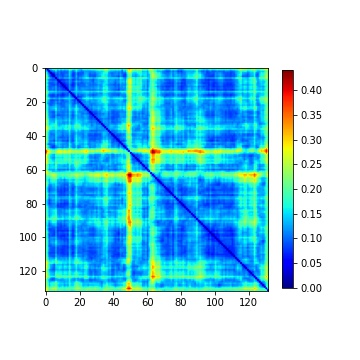
\includegraphics[width=10cm]{figures/cohort_distance_all.jpg}
\caption{Pairwise Hamming distance between the decisions on treatment of a standard cohort of 10,000 patients made at each hospital.}
\label{fig:cohort_distance_all}
\end{figure}

% \begin{figure}[h]
% \centering
% 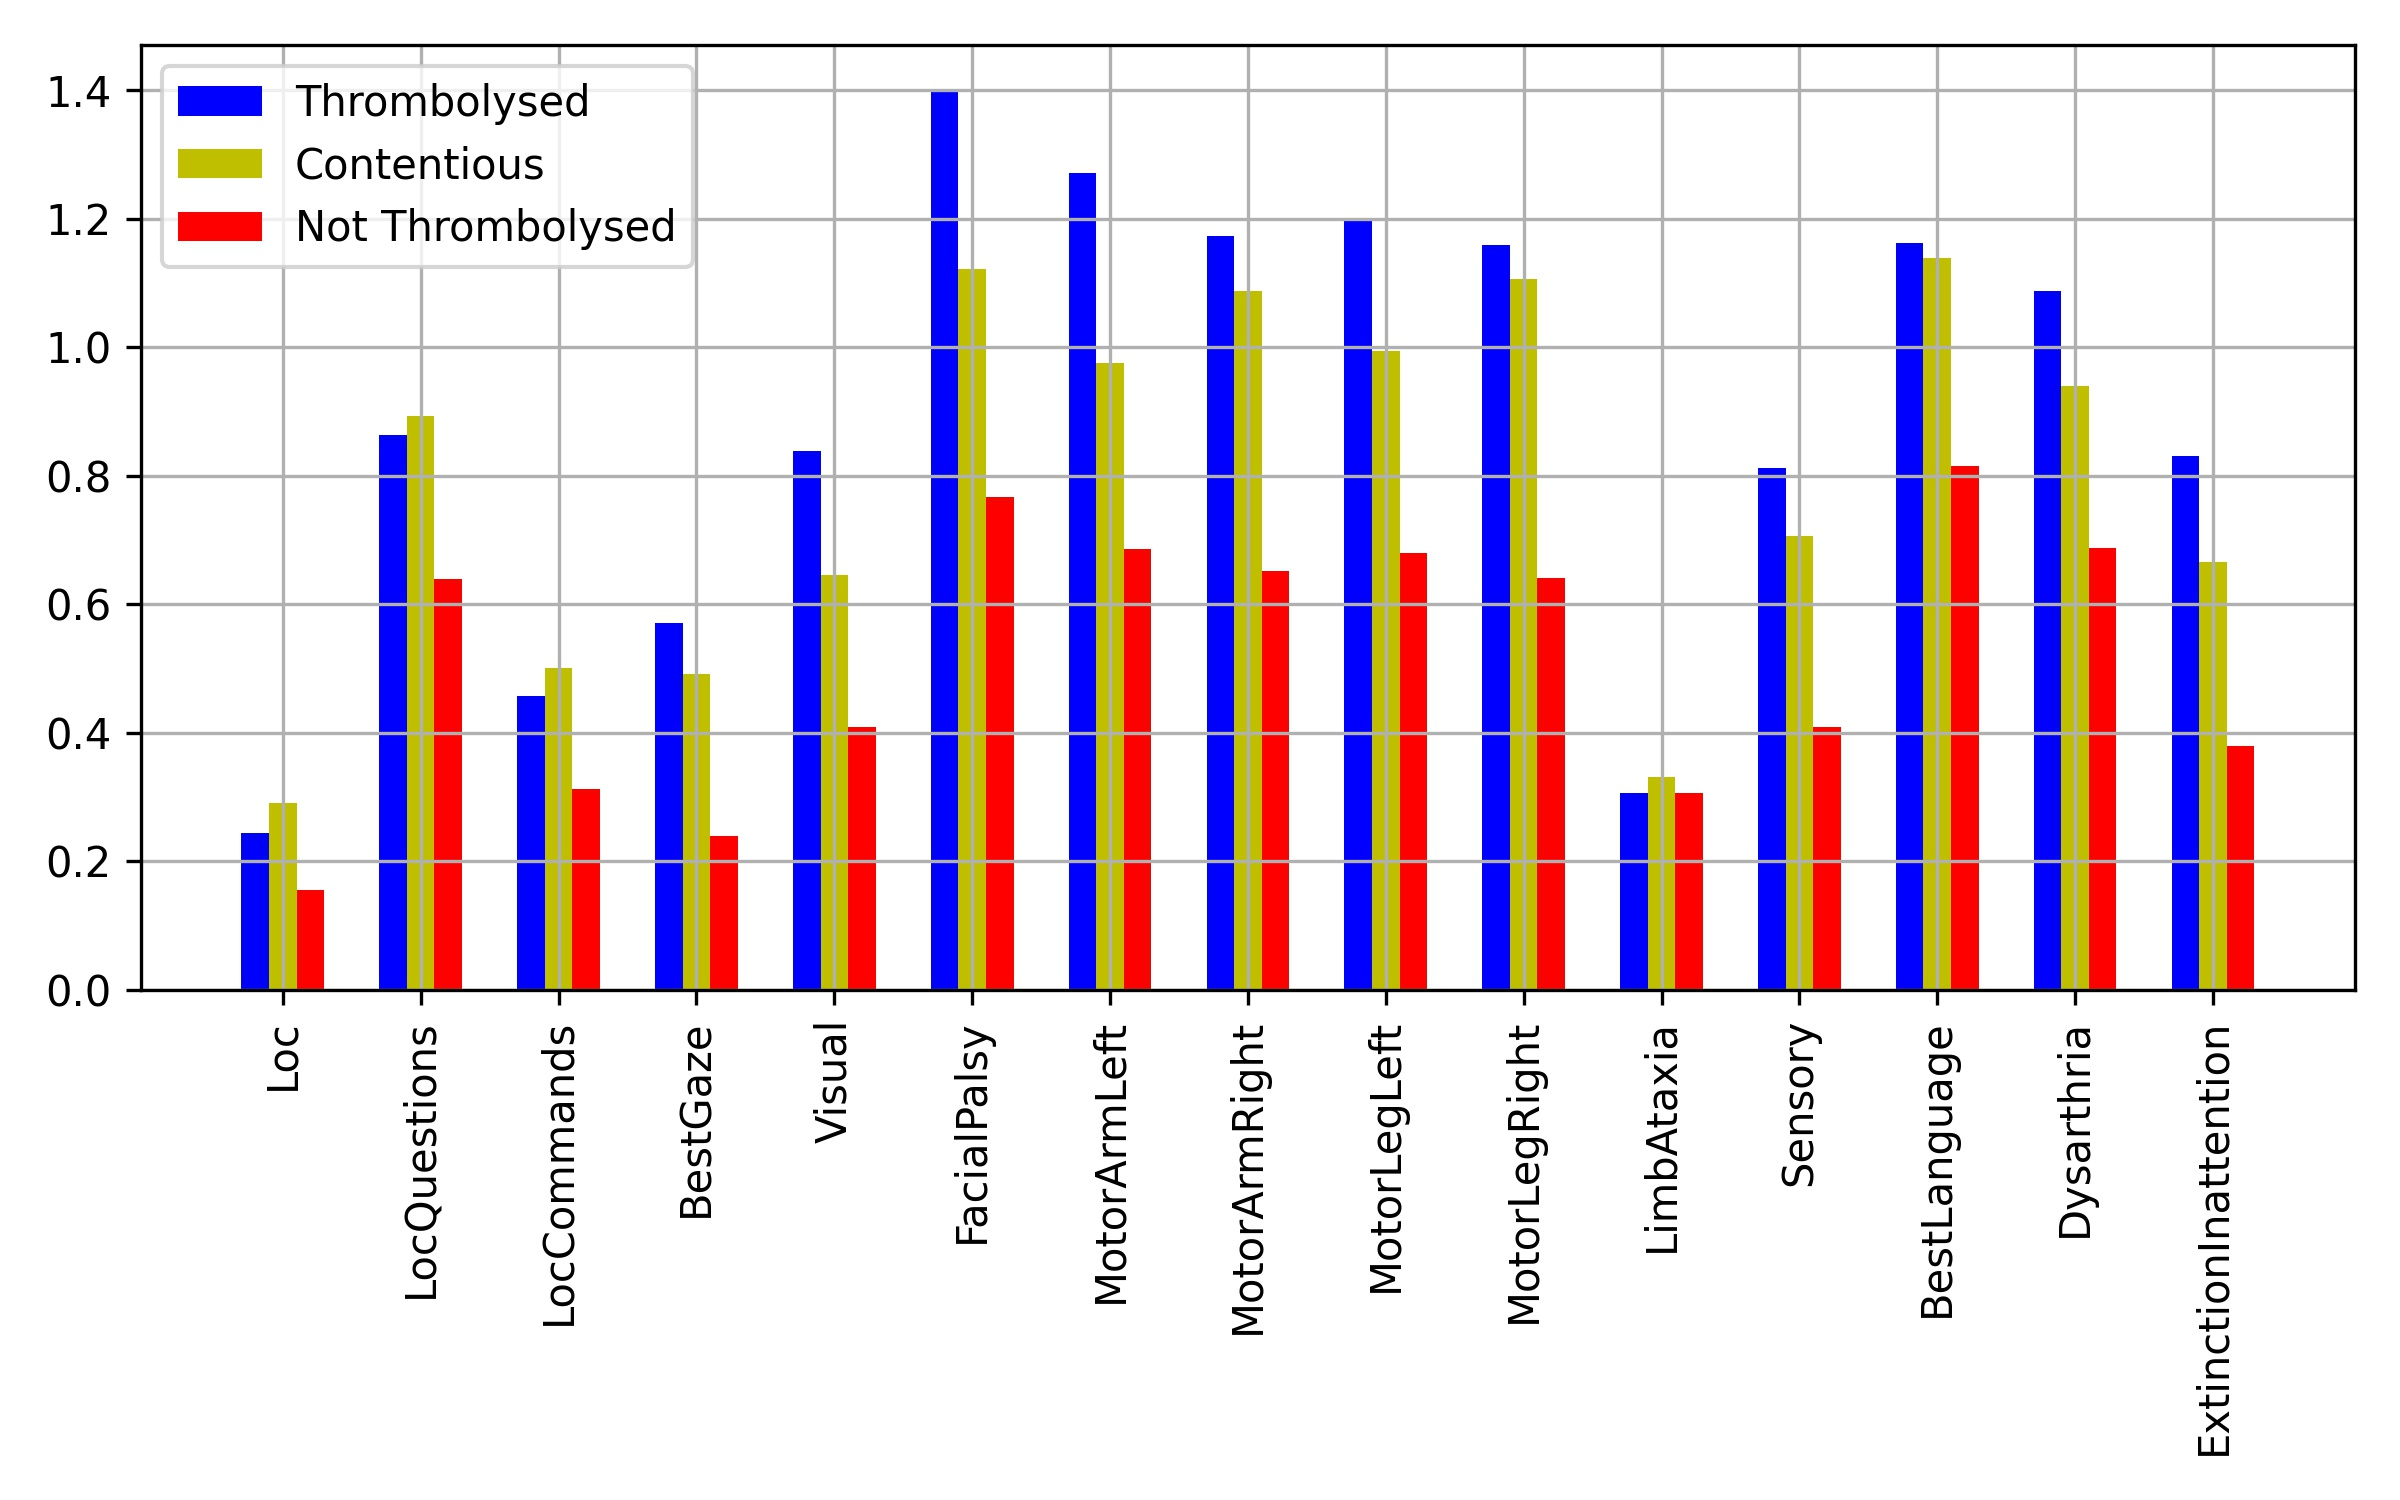
\includegraphics[width=15cm]{figures/contentious_nihss.jpg}
% \caption{}
% \label{fig:cohort_nihss}
% \end{figure}


\end{document}

%%% Local Variables:
%%% mode: latex
%%% TeX-master: t
%%% End:
